\documentclass[conference]{IEEEtran}

\IEEEoverridecommandlockouts
% The preceding line is only needed to identify funding in the first footnote. If that is unneeded, please comment it out.
\usepackage{cite}
\usepackage{amsmath,amssymb,amsfonts}
\usepackage{algorithmic}
\usepackage{graphicx}
\usepackage{textcomp}
\def\BibTeX{{\rm B\kern-.05em{\sc i\kern-.025em b}\kern-.08em
    T\kern-.1667em\lower.7ex\hbox{E}\kern-.125emX}}
\usepackage[utf8]{inputenc}
\usepackage[spanish]{babel}

\usepackage{multirow}
\usepackage[table,xcdraw]{xcolor} % Tablas

\usepackage{minted}

\usepackage{cuted}

\usepackage{url}

\usepackage{listings} % Código

%\usepackage{subfig}

\lstset{literate=
  {á}{{\'a}}1 {é}{{\'e}}1 {í}{{\'i}}1 {ó}{{\'o}}1 {ú}{{\'u}}1
  {Á}{{\'A}}1 {É}{{\'E}}1 {Í}{{\'I}}1 {Ó}{{\'O}}1 {Ú}{{\'U}}1
  {à}{{\`a}}1 {è}{{\`e}}1 {ì}{{\`i}}1 {ò}{{\`o}}1 {ù}{{\`u}}1
  {À}{{\`A}}1 {È}{{\'E}}1 {Ì}{{\`I}}1 {Ò}{{\`O}}1 {Ù}{{\`U}}1
  {ä}{{\"a}}1 {ë}{{\"e}}1 {ï}{{\"i}}1 {ö}{{\"o}}1 {ü}{{\"u}}1
  {Ä}{{\"A}}1 {Ë}{{\"E}}1 {Ï}{{\"I}}1 {Ö}{{\"O}}1 {Ü}{{\"U}}1
  {â}{{\^a}}1 {ê}{{\^e}}1 {î}{{\^i}}1 {ô}{{\^o}}1 {û}{{\^u}}1
  {Â}{{\^A}}1 {Ê}{{\^E}}1 {Î}{{\^I}}1 {Ô}{{\^O}}1 {Û}{{\^U}}1
  {Ã}{{\~A}}1 {ã}{{\~a}}1 {Õ}{{\~O}}1 {õ}{{\~o}}1
  {œ}{{\oe}}1 {Œ}{{\OE}}1 {æ}{{\ae}}1 {Æ}{{\AE}}1 {ß}{{\ss}}1
  {ű}{{\H{u}}}1 {Ű}{{\H{U}}}1 {ő}{{\H{o}}}1 {Ő}{{\H{O}}}1
  {ç}{{\c c}}1 {Ç}{{\c C}}1 {ø}{{\o}}1 {å}{{\r a}}1 {Å}{{\r A}}1
  {€}{{\euro}}1 {£}{{\pounds}}1 {«}{{\guillemotleft}}1
  {»}{{\guillemotright}}1 {ñ}{{\~n}}1 {Ñ}{{\~N}}1 {¿}{{?`}}1
}

\definecolor{mGreen}{rgb}{0,0.6,0}
\definecolor{mGray}{rgb}{0.5,0.5,0.5}
\definecolor{mPurple}{rgb}{0.58,0,0.82}
\definecolor{backgroundColour}{rgb}{0.95,0.95,0.92}

\lstdefinestyle{CStyle}{
    backgroundcolor=\color{backgroundColour},   
    commentstyle=\color{mGreen},
    keywordstyle=\color{magenta},
    numberstyle=\tiny\color{mGray},
    stringstyle=\color{mPurple},
    basicstyle=\scriptsize\ttfamily,
    breakatwhitespace=false,         
    breaklines=true,                 
    captionpos=b,                    
    keepspaces=true,                 
    numbers=left,                    
    numbersep=5pt,                  
    showspaces=false,                
    showstringspaces=false,
    showtabs=false,                  
    tabsize=2,
    language=C
}

\lstdefinestyle{customasm}{
  backgroundcolor=\color{backgroundColour},   
    %commentstyle=\color{mGreen},
    keywordstyle=\color{magenta},
    numberstyle=\tiny\color{mGray},
    stringstyle=\color{mPurple},
    basicstyle=\footnotesize,
    breakatwhitespace=false,         
    breaklines=true,                 
    captionpos=b,                    
    keepspaces=true,                 
    numbers=left,                    
    numbersep=5pt,                  
    showspaces=false,                
    showstringspaces=false,
    showtabs=false,                  
    tabsize=2,
  language=[x86masm]Assembler
}

\begin{document}

\def\UrlBreaks{\do\/\do-\do\_} % Para que las URLs no sobrepasen (generalmente) una columna en longitud

\title{Multiplicación de cuaterniones mediante programación multinúcleo y extensiones SSE\\
%{\footnotesize \textsuperscript{*}Note: Sub-titles are not captured in Xplore and
%should not be used}
%\thanks{Identify applicable funding agency here. If none, delete this.}
}

\author{\IEEEauthorblockN{Álvaro Goldar Dieste}
\IEEEauthorblockA{\textit{Universidad de Santiago de Compostela} \\
%%\textit{name of organization (of Aff.)}\\
Santiago de Compostela, España \\
alvaro.goldar@rai.usc.es}
\and
\IEEEauthorblockN{Francisco Javier Cardama Santiago}
\IEEEauthorblockA{\textit{Universidad de Santiago de Compostela} \\
%\textit{name of organization (of Aff.)}\\
Santiago de Compostela, España \\
franciscojavier.cardama@rai.usc.es}
}

\maketitle

% Insertar tras maketitle para mostrar los números de página
\thispagestyle{plain}
\pagestyle{plain}

\begin{abstract}
En este documento se tratan las ventajas que aporta la programación multinúcleo y extensiones SSE en la eficiencia de grandes cómputos.

Se implementarán distintas soluciones utilizando diversas técnicas para determinar el coste temporal de un bucle computacional que consta de operaciones sobre vectores de cuaterniones. Concretamente, se empleará la programación multihilo mediante OpenMP, y la programación vectorial mediante el uso de extensiones SIMD.

Mediante estos experimentos se concluirá que la programación multinúcleo beneficia notablemente la rapidez del cómputo generalmente, mientras que las extensiones SIMD, si no se aplican correctamente, pueden llegar a penalizar los resultados.

\textbf{\textit{Palabras clave}---OpenMP, SSE, SIMD, multihilo, cuaternión}
\end{abstract}

%\begin{IEEEkeywords}
%component, formatting, style, styling, insert
%\end{IEEEkeywords}

\section{Introducción}

En este informe se tratarán diversos experimentos en los que, en cada uno de ellos, se determina el coste temporal de un bucle de computación, el cual consta de operaciones sobre vectores de cuaterniones, para realizar una comparativa de las ventajas y desventajas de determinadas técnicas de programación en función del proceso de implementación y de los resultados obtenidos para cada una. Entre ellas se incluirán la programación multihilo y las extensiones SSE.

Estos experimentos serán llevados a cabo sobre un computador en específico, cuyas especificaciones de interés se encuentran descritas en la Sección \ref{descripcionComputador}.

Para ello, se explicarán previamente en la Sección \ref{descripcionMultiplicacionCuaterniones} las distintas operaciones que se pueden realizar con los cuaterniones y sus propiedades más importantes para el desarrollo del informe.

Todas estas explicaciones se verán reflejadas en la Sección \ref{tipoExperimento}, donde se mostrarán las diversas implementaciones desarrolladas en el lenguaje de programación \textit{\textbf{C}} para los experimentos descritos. Para analizar el rendimiento de una parte de las implementaciones llevadas a cabo, en la sección \ref{IACA} se utilizará la herramienta \textit{Intel Architecture Code Analyzer (IACA)}.

En la Sección \ref{experimentos} se detallará cómo se realizarán los experimentos y, posteriormente, en la Sección \ref{resumenExperimentos} se tratarán los resultados obtenidos para las previas implementaciones.

Por último se realizará un análisis seguido de una breve reflexión sobre la eficiencia de las soluciones implementadas la Sección \ref{conclusiones}.

\section{Operaciones con cuaterniones} \label{descripcionMultiplicacionCuaterniones}

En el informe se estudiarán los ciclos empleados en el cómputo de determinadas operaciones con cuaterniones, que son una extensión de los números reales. Abstrayéndose del ámbito matemático, a la hora de representar su información se tratarán como vectores de cuatro términos.

\begin{center}
    $a = (a_{0}, a_{1}, a_{2}, a_{3})$
\end{center}

Las operaciones que serán necesarias para este experimento son la \textbf{adición} y el \textbf{producto}.

La \textbf{\textit{adición}} de cuaterniones se realiza de término a término de forma que, si se tienen los siguientes valores,

\begin{equation*}
    a = (a_{0}, a_{1}, a_{2}, a_{3})
\end{equation*}
\begin{equation*}
    b = (b_{0}, b_{1}, b_{2}, b_{3}),
\end{equation*}

la suma resultante sería la suma término a término

\begin{center}
    $a + b= (a_{0} + b_{0}, a_{1} + b_{1}, a_{2} + b_{2}, a_{3} + b_{3})$.
\end{center}

Las propiedades de la suma en los cuaterniones son equivalentes a la de la suma matricial o de números reales. Las más importantes para el experimento serán la \textit{conmutativa} y la \textit{asociativa}.

Por otra parte, otra de las operaciones que será necesarias para el cómputo es el \textit{\textbf{producto}} entre cuaterniones. La expresión del producto de forma matemática es la siguiente \cite{paperOperacionesCuaterniones}.

\begin{equation*}
    a\cdot b = (\alpha \cdot \beta - \vec{a} \cdot \vec{b}, \alpha \cdot \vec{b} + \beta \cdot \vec{a} + \vec{a} \times \vec{b}),
\end{equation*}

de forma que los valores intermedios utilizados son
\begin{equation*}
    \alpha = a_{0},
\end{equation*}
\begin{equation*}
    \beta = b_{0},
\end{equation*}
\begin{equation*}
    \vec{a} = (a_{1}, a_{2}, a_{3}),
\end{equation*}
\begin{equation*}
    \vec{b} = (b_{1}, b_{2}, b_{3}).
\end{equation*}

En la Ecuación \ref{productoCuat} se obtiene la expresión de la multiplicación de cuaterniones para cada término empleando exclusivamente operaciones de números reales.
\begin{equation}
    \label{productoCuat}
    c = a\cdot b = (c_{0}, c_{1}, c_{2}, c_{3}),
\end{equation}
\begin{equation*}
    c_{0} = a_{0} \cdot b_{0} - a_{1} \cdot b_{1} - a_{2} \cdot b_{2} - a_{3} \cdot b_{3},
\end{equation*}
\begin{equation*}
    c_{1} = a_{0} \cdot b_{1} + a_{1} \cdot b_{0} + a_{2} \cdot b_{3} - a_{3} \cdot b_{2},
\end{equation*}
\begin{equation*}
    c_{2} = a_{0} \cdot b_{2} - a_{1} \cdot b_{3} + a_{2} \cdot b_{0} + a_{3} \cdot b_{1},
\end{equation*}
\begin{equation*}
    c_{3} = a_{0} \cdot b_{3} + a_{1} \cdot b_{2} - a_{2} \cdot b_{1} + a_{3} \cdot b_{0}.
\end{equation*}

Respecto al producto, es interesante comentar que, al igual que el producto matricial, el producto de cuaterniones es asociativo pero no conmutativo, lo cual será necesario tener en cuenta a la hora de realizar una programación de dicho producto.

Por otro lado, es interesante comentar la multiplicación de dos cuaterniones iguales, debido a que se puede deducir una expresión más simplificada que requiera menos operaciones que la multiplicación de la Ecuación \ref{productoCuat}.

Si se realiza dicha operación, se obtendría el siguiente resultado final:

\begin{equation}
    \label{productoCuatIguales1}
    c = a\cdot a = (c_{0}, c_{1}, c_{2}, c_{3}),
\end{equation}
\begin{equation*}
    c_{0} = a_{0} \cdot a_{0} - a_{1} \cdot a_{1} - a_{2} \cdot a_{2} - a_{3} \cdot a_{3},
\end{equation*}
\begin{equation*}
    c_{1} = a_{0} \cdot a_{1} + a_{1} \cdot a_{0} + a_{2} \cdot a_{3} - a_{3} \cdot a_{2},
\end{equation*}
\begin{equation*}
    c_{2} = a_{0} \cdot a_{2} - a_{1} \cdot a_{3} + a_{2} \cdot a_{0} + a_{3} \cdot a_{1},
\end{equation*}
\begin{equation*}
    c_{3} = a_{0} \cdot a_{3} + a_{1} \cdot a_{2} - a_{2} \cdot a_{1} + a_{3} \cdot a_{0}.
\end{equation*}

Y, como el cuaternión está compuesto por números reales y el producto de estos es conmutativo, se obtendría la siguiente expresión simplificada:

\begin{equation}
    \label{productoCuatIguales2}
    c = a\cdot a = (c_{0}, c_{1}, c_{2}, c_{3}),
\end{equation}
\begin{equation*}
    c_{0} = a_{0} \cdot a_{0} - a_{1} \cdot a_{1} - a_{2} \cdot a_{2} - a_{3} \cdot a_{3},
\end{equation*}
\begin{equation*}
    c_{1} = 2 \cdot a_{0} \cdot a_{1},
\end{equation*}
\begin{equation*}
    c_{2} = 2 \cdot a_{0} \cdot a_{2},
\end{equation*}
\begin{equation*}
    c_{3} = 2 \cdot a_{0} \cdot a_{3}.
\end{equation*}

\section{Computador empleado en los experimentos} \label{descripcionComputador}

Para este experimento, se emplearán los servicios del Finisterrae II del Centro de Supercomputación de Galicia \cite{cesga}.

\subsection{Especificaciones del procesador}

Concretamente, cada experimento será ejecutado sobre un nodo que pone a disposición un procesador Intel Xeon E5-2650 v3 \cite{procesador}. Este dispone, entre otras, de las siguientes características:
\begin{itemize}
    \item Frecuencia de 2.30 GHz.
    \item 10 cores con soporte cada uno para 2 hilos.
    \item Caché L3 de datos de 25 MB compartida entre todos los cores.
    \item Cache L1 de instrucciones de 32 KB privada para cada core.
    \item Soporte para instrucciones SSE, SSE2 y SSE3, las cuales serán empleadas para la programación SIMD.
\end{itemize}

\subsection{Sistema Operativo}

Cada uno de los nodos candidatos ofrece el sistema operativo Linux para cada uno de los trabajos que se ejecutan sobre ellos. Además, se emplearán las dos siguientes herramientas, pertenecientes a la suite de Intel para desarrolladores, al haberse fijado un determinado procesador sobre el que ejecutar los experimentos:
\begin{itemize}
    \item El compilador ICC \cite{icc}.
    \item El analizador IACA \cite{iacaDescarga}. 
\end{itemize}
El motivo por el cual se ha empleado esta última utilidad se detallará más adelante.

\section{Programas de pruebas} \label{tipoExperimento}
Para comparar los tiempos obtenidos al realizar operaciones sobre cuaterniones en distintos programas de prueba, se abordará un problema en específico que consistirá en calcular un cuaternión final $dp$ mediante unas operaciones determinadas.

Las entradas son dos vectores de cuaterniones de tamaño $N$: $a(N), b(N)$, inicializados con valores aleatorios. En un experimento dado, $N$ se calculará de forma que $N = 10^{q}$, probando los valores $q = \{2, 4, 6, 7, 8\}$.

Con estos vectores se realizará la multiplicación de los cuaterniones anteriores y se almacenará en un vector auxiliar $c(N)$

\begin{equation*}
    c(i) = a(i) \cdot b(i).
\end{equation*}

Posteriormente, una vez realizada la multiplicación de los cuaterniones de $a$ y de $b$, se realizará una reducción en $dp$

\begin{equation*}
    dp = dp + c(i) \cdot c(i).
\end{equation*}

Por lo tanto, para abordar este problema, se estudiarán distintos tipos de soluciones en el lenguaje de programación \textbf{\textit{C}}. La primera de ellas será realizar la implementación directa del algoritmo, obteniendo un código \textit{secuencial}, dando lugar posteriormente a una segunda, con un código \textit{secuencial optimizado}. Tras ello, se pasará a aprovechar la programación vectorial mediante extensiones SSE, vectorizando en una implementación la \textit{multiplicación} de cuaterniones y, en la otra, el \textit{bucle computacional}. Por último, se aprovechará la programación multihilo con \textit{\textbf{OpenMP}} para paralelizar el cómputo. Tanto la programación vectorial como la multihilo tomarán como base la versión secuencial optimizada del código.

\subsection{Implementaciones secuenciales}

Como se explicó previamente, el primer código a realizar se trata del secuencial sin optimizaciones. Este se dispone a continuación.

\begin{lstlisting}[style=CStyle, title=Código secuencial sin optimizaciones.]
#include <stdio.h>
#include <stdlib.h>
#include <math.h>
#include <time.h>
#include <unistd.h>
#include <pmmintrin.h>


// Múltiplo del que tienen que ser las direcciones de
// memoria a reservar para un alineado correcto para SIMD
#define ALIN_MULT 16

/* Macros varias */
#define FALSE 0
#define TRUE 1


/* Prototipos de las funciones a emplear */
void inicializarVectorCuaternion( float **vector, size_t
    numElementos, int valoresAleatorios );
void liberarVectorCuaternion( float **vector );

void productoCuaterniones( float *operando1, float
    *operando2, float *destino );

void productoSumaCuaterniones( float *operando1, float
    *operando2, float *destino );


/* Main */

int main(int argc, char **argv)
{
    /* Variables a emplear */

    // Número de cuaterniones contenidos en cada array
    size_t n;

    // Orden de magnitud del tamaño de los vectores de
    // input
    size_t q;

    // Vectores de cuaterniones de valores aleatorios
    // (input)
    float *a;
    float *b;

    // Vector auxiliar de cuaterniones
    float *c;

    // Cuaternión sobre el que realizar la computación
    // (output)
    float dp[ 4 ];

    // Variable sobre la que contabilizar el tiempo
    // transcurrido
    double ck;

    // Contadores
    int i;


    /***** Argumentos *****/

    if( argc < 2 )
    {
        printf( "Número de valores incorrecto. Uso: %s "
            "<q>\n", argv[ 0 ] );
        exit( EXIT_FAILURE );
    }

    // Se obtiene el valor de 'q' dado
    q = atoi( argv[ 1 ] );

    if( q <= 0 )
    {
        printf( "El valor de q debe ser mayor que 0\n" );
        exit( EXIT_FAILURE );
    }


    /***** Inicialización *****/

    // Se obtiene una semilla para la generación de números
    // aleatorios
    srand( ( unsigned )time( NULL ) );

    // Se calcula el tamaño final de los vectores de input
    n = ( int )pow( 10, q );

    // Se inicializan los vectores de cuaterniones
    inicializarVectorCuaternion( &a, n, TRUE );
    inicializarVectorCuaternion( &b, n, TRUE );
    inicializarVectorCuaternion( &c, n, FALSE );


    /***** Computación *****/

    // Se inicia el medidor de tiempo
    ck = 0;
    start_counter();

    // Se almacena en el vector 'c' la multiplicación de
    // los vectores 'a' y 'b'
    for( i = 0; i < n; i++ )
    {
        productoCuaterniones( a + i * 4, b + i * 4, c + i *
            4 );
    }

    // Se inicializan los valores del cuaternión 'dp' a '0'
    dp[ 0 ] = 0;
    dp[ 1 ] = 0;
    dp[ 2 ] = 0;
    dp[ 3 ] = 0;

    // Se realiza sobre el cuaternión 'dp' la suma de la
    // multiplicación de cada cuaternión del vector 'c' por
    // sí mismo
    for( i = 0; i < n; i++ )
    {
        productoSumaCuaterniones( c + i * 4, c + i * 4,
            dp );
    }

    // Se finaliza el medidor de tiempo
    ck = get_counter();

    printf( "%d,%lu,%1.10lf\n", atoi( argv[ 2 ] ), q, ck );
    
    printf( "Resultado: [%f, %f, %f, %f]\n", dp[ 0 ],
        dp[ 1 ], dp[ 2 ], dp[ 3 ] );

    // Se libera la memoria reservada
    liberarVectorCuaternion( &a );
    liberarVectorCuaternion( &b );
    liberarVectorCuaternion( &c );


    return( EXIT_SUCCESS );
}


void inicializarVectorCuaternion( float **vector, size_t
    numElementos, int valoresAleatorios )
{
    // Contador
    int i;


    // Se reserva la memoria necesaria para el vector de cuaterniones
    if( ( *vector = _mm_malloc( numElementos * 4 *
        sizeof( float ), ALIN_MULT ) ) == NULL )
    {
        perror( "Reserva de memoria del vector de "
            "cuaterniones fallida" );
        exit( EXIT_FAILURE );
    }

    if( valoresAleatorios == TRUE )
    {
        // Y se genera en cada posición de los cuaterniones
        // de los vectores un valor entre 1 y 2
        for( i = 0; i < numElementos; i++ )
        {
            *( *vector + i * 4 ) = ( ( double )rand() /
                RAND_MAX + 1 ) * pow( -1, rand() % 2 );
            *( *vector + i * 4 + 1 ) = ( ( double )rand() /
                RAND_MAX + 1 ) * pow( -1, rand() % 2 );
            *( *vector + i * 4 + 2 ) = ( ( double )rand() /
                RAND_MAX + 1 ) * pow( -1, rand() % 2 );
            *( *vector + i * 4 + 3 ) = ( ( double )rand() /
                RAND_MAX + 1 ) * pow( -1, rand() % 2 );
        }
    }

    else
    {
        // En caso contrario, se inicializan los valores a
        // '0'
        for( i = 0; i < numElementos; i++ )
        {
            *( *vector + i * 4 ) = 0;
            *( *vector + i * 4 + 1 ) = 0;
            *( *vector + i * 4 + 2 ) = 0;
            *( *vector + i * 4 + 3 ) = 0;
        }
    }
}


void liberarVectorCuaternion( float **vector )
{
    _mm_free( *vector );
}


void productoCuaterniones( float *operando1, float
    *operando2, float *destino )
{
    destino[ 0 ] = operando1[ 0 ] * operando2[ 0 ] -
        operando1[ 1 ] * operando2[ 1 ] - operando1[ 2 ] *
        operando2[ 2 ] - operando1[ 3 ] * operando2[ 3 ];

    destino[ 1 ] = operando1[ 0 ] * operando2[ 1 ] +
        operando1[ 1 ] * operando2[ 0 ] + operando1[ 2 ] *
        operando2[ 3 ] - operando1[ 3 ] * operando2[ 2 ];

    destino[ 2 ] = operando1[ 0 ] * operando2[ 2 ] -
        operando1[ 1 ] * operando2[ 3 ] + operando1[ 2 ] *
        operando2[ 0 ] + operando1[ 3 ] * operando2[ 1 ];

    destino[ 3 ] = operando1[ 0 ] * operando2[ 3 ] +
        operando1[ 1 ] * operando2[ 2 ] - operando1[ 2 ] *
        operando2[ 1 ] + operando1[ 3 ] * operando2[ 0 ];
}


void productoSumaCuaterniones( float *operando1, float
    *operando2, float *destino )
{
    destino[ 0 ] += operando1[ 0 ] * operando2[ 0 ] -
        operando1[ 1 ] * operando2[ 1 ] - operando1[ 2 ] *
        operando2[ 2 ] - operando1[ 3 ] * operando2[ 3 ];

    destino[ 1 ] += operando1[ 0 ] * operando2[ 1 ] +
        operando1[ 1 ] * operando2[ 0 ] + operando1[ 2 ] *
        operando2[ 3 ] - operando1[ 3 ] * operando2[ 2 ];

    destino[ 2 ] += operando1[ 0 ] * operando2[ 2 ] -
        operando1[ 1 ] * operando2[ 3 ] + operando1[ 2 ] *
        operando2[ 0 ] + operando1[ 3 ] * operando2[ 1 ];

    destino[ 3 ] += operando1[ 0 ] * operando2[ 3 ] +
        operando1[ 1 ] * operando2[ 2 ] - operando1[ 2 ] *
        operando2[ 1 ] + operando1[ 3 ] * operando2[ 0 ];
}
\end{lstlisting}

Como se puede observar, en él se ha realizado una traducción directa de las operaciones $c(i) = a(i) \cdot b(i)$ y $dp = dp + c(i) \cdot c(i)$ en la forma de las funciones \texttt{productoCuaterniones} y \texttt{productoSumaCuaterniones} respectivamente, empleando las correspondientes instrucciones del lenguaje C con las que replicar las expresiones mostradas en la Sección \ref{productoCuat}. Por ello, teniendo en cuenta además la documentación disponible sobre el funcionamiento del programa, como la generación aleatoria de valores para los vectores de cuaterniones $a$ y $b$, no se redundará más en este código y se procederá a explicar la versión secuencial optimizada.

El código de la versión optimizada puede verse a continuación.

\begin{lstlisting}[style=CStyle, title=Código secuencial optimizado.]
#include <stdio.h>
#include <stdlib.h>
#include <math.h>
#include <time.h>
#include <unistd.h>
#include <pmmintrin.h>


// Múltiplo del que tienen que ser las direcciones de memoria a reservar para
// un alineado correcto para SIMD
#define ALIN_MULT 16

/* Macros varias */
#define FALSE 0
#define TRUE 1


/* Prototipos de las funciones a emplear */
void inicializarVectorCuaternion( float **vector, size_t
    numElementos, int valoresAleatorios );
void liberarVectorCuaternion( float **vector );


/* Main */

int main(int argc, char **argv)
{
    /* Variables a emplear */

    // Número de cuaterniones contenidos en cada array
    size_t n;

    // Orden de magnitud del tamaño de los vectores de
    // input
    size_t q;

    // Vectores de cuaterniones de valores aleatorios
    // (input)
    float *a;
    float *b;

    // Vector auxiliar de cuaterniones
    float *c;

    // Cuaternión sobre el que realizar la computación
    // (output)
    float dp[ 4 ] = { 0, 0, 0, 0 };

    // Variable sobre la que contabilizar el tiempo transcurrido
    // 
    double ck;

    // Variables auxiliares en las que almacenar elementos
    // de cuaterniones
    float a0, a1, a2, a3, b0, b1, b2, b3, c0, c1, c2, c3;

    // Contadores
    int i;


    /***** Argumentos *****/

    if( argc < 2 )
    {
        printf( "Número de valores incorrecto. Uso: %s "
            "<q>\n", argv[ 0 ] );
        exit( EXIT_FAILURE );
    }

    // Se obtiene el valor de 'q' dado
    q = atoi( argv[ 1 ] );

    if( q <= 0 )
    {
        printf( "El valor de q debe ser mayor que 0\n" );
        exit( EXIT_FAILURE );
    }


    /***** Inicialización *****/

    // Se obtiene una semilla para la generación de números
    // aleatorios
    srand( ( unsigned )time( NULL ) );

    // Se calcula el tamaño final de los vectores de input
    n = ( int )pow( 10, q );

    // Se inicializan los vectores de cuaterniones
    inicializarVectorCuaternion( &a, n, TRUE );
    inicializarVectorCuaternion( &b, n, TRUE );
    inicializarVectorCuaternion( &c, n, FALSE );
    

    /***** Computación *****/

    // Se inicia el medidor de tiempo
    ck = 0;
    start_counter();

    // Se almacena en el vector 'c' la multiplicación de
    // los vectores 'a' y 'b'
    for( i = 0; i < n; i++ )
    {
        // Se guardan las componentes de los cuaterniones
        // iterados
        a0 = *( a + i * 4 );
        a1 = *( a + i * 4 + 1 );
        a2 = *( a + i * 4 + 2 );
        a3 = *( a + i * 4 + 3 );

        b0 = *( b + i * 4 );
        b1 = *( b + i * 4 + 1 );
        b2 = *( b + i * 4 + 2 );
        b3 = *( b + i * 4 + 3 );

        // Se realiza el producto del primer cuaternión por
        // el segundo
        *( c + i * 4 ) = a0 * b0 - a1 * b1 - a2 * b2 - a3
            * b3;
        *( c + i * 4 + 1 ) = a0 * b1 + a1 * b0 + a2 * b3 -
            a3 * b2;
        *( c + i * 4 + 2 ) = a0 * b2 - a1 * b3 + a2 * b0 +
            a3 * b1;
        *( c + i * 4 + 3 ) = a0 * b3 + a1 * b2 - a2 * b1 +
            a3 * b0;
    }

    // Se realiza sobre el cuaternión 'dp' la suma de la
    // multiplicación de cada cuaternión del vector 'c' por
    // sí mismo
    for( i = 0; i < n; i++ )
    {
        // Se guardan las componentes del cuaternión
        // iterado
        c0 = *( c + i * 4 );
        c1 = *( c + i * 4 + 1 );
        c2 = *( c + i * 4 + 2 );
        c3 = *( c + i * 4 + 3 );

        // Se realiza el producto del primer cuaternión por
        // el segundo
        dp[ 0 ] += c0 * c0 - c1 * c1 - c2 * c2 - c3 * c3;
        dp[ 1 ] += ( c0 + c0 ) * c1;
        dp[ 2 ] += ( c0 + c0 ) * c2;
        dp[ 3 ] += ( c0 + c0 ) * c3;
    }

    // Se finaliza el medidor de tiempo
    ck = get_counter();

    printf( "%d,%lu,%1.10lf\n", atoi( argv[ 2 ] ), q, ck );
    
    printf( "Resultado: [%f, %f, %f, %f]\n", dp[ 0 ],
        dp[ 1 ], dp[ 2 ], dp[ 3 ] );

    // Se libera la memoria reservada
    liberarVectorCuaternion( &a );
    liberarVectorCuaternion( &b );
    liberarVectorCuaternion( &c );


    return( EXIT_SUCCESS );
}


void inicializarVectorCuaternion( float **vector, size_t
    numElementos, int valoresAleatorios )
{
    // Contador
    int i;


    // Se reserva la memoria necesaria para el vector de
    // cuaterniones
    if( ( *vector = _mm_malloc( numElementos * 4 *
        sizeof( float ), ALIN_MULT ) ) == NULL )
    {
        perror( "Reserva de memoria del vector de "
            "cuaterniones fallida" );
        exit( EXIT_FAILURE );
    }

    if( valoresAleatorios == TRUE )
    {
        // Y se genera en cada posición de los cuaterniones
        // de los vectores un valor entre 1 y 2
        for( i = 0; i < numElementos; i++ )
        {
            *( *vector + i * 4 ) = ( ( double )rand() /
                RAND_MAX + 1 ) * pow( -1, rand() % 2 );
            *( *vector + i * 4 + 1 ) = ( ( double )rand() /
                RAND_MAX + 1 ) * pow( -1, rand() % 2 );
            *( *vector + i * 4 + 2 ) = ( ( double )rand() /
                RAND_MAX + 1 ) * pow( -1, rand() % 2 );
            *( *vector + i * 4 + 3 ) = ( ( double )rand() /
                RAND_MAX + 1 ) * pow( -1, rand() % 2 );
        }
    }

    else
    {
        // En caso contrario, se inicializan los valores a
        // '0'
        for( i = 0; i < numElementos; i++ )
        {
            *( *vector + i * 4 ) = 0;
            *( *vector + i * 4 + 1 ) = 0;
            *( *vector + i * 4 + 2 ) = 0;
            *( *vector + i * 4 + 3 ) = 0;
        }
    }
}


void liberarVectorCuaternion( float **vector )
{
    _mm_free( *vector );
}
\end{lstlisting}

Puede verse en este caso cómo se han realizado una serie de sencillos cambios para tratar de reducir el número de ciclos empleados en la sección computacional.

El primer cambio, aunque prácticamente insignificante, consiste en la inicialización de $dp$ a $(0, 0, 0, 0)$ en su misma declaración, en lugar de hacerlo dentro de la sección del cómputo.

El segundo cambio consiste en la eliminación de las funciones para realizar los cómputos de ambos bucles, incorporando en su lugar las instrucciones correspondientes en ellos. De este modo, se evita el \textit{overhead} producido por la necesidad de efectuar constantemente llamadas a funciones.

El tercer cambio se trata de, en cada bucle, almacenar en variables auxiliares los operandos a emplear en los cálculos en lugar de referenciarlos constantemente mediante direcciones de memoria. De este modo se conseguirá mejorar, por lo menos, levemente el rendimiento del programa, dado que es probable que, en caso de no haberlo tenido en cuenta, el procesador probablemente no se vería muy perjudicado como consecuencia del principio de localidad y de sus mecanismos de predicción de uso de datos.

Y el cuarto y último cambio se trata de una optimización que es posible efectuar sobre el segundo bucle como consecuencia de calcular la multiplicación del cuaternión $c$ por sí mismo. Tomando como referencia la Ecuación \ref{productoCuatIguales2}, el tomar un único cuaternión como ambos operandos permite simplificar en gran medida el cálculo del producto, tal y como se puede ver en el código secuencial optimizado. Esto implica directamente una clara reducción del número de instrucciones que el procesador debe llevar a cabo en cada iteración del segundo bucle, y que probablemente se hará notar en el rendimiento global de este programa.

\subsection{Implementaciones vectorizadas}

Para realizar las implementaciones vectorizadas, será necesario incluir la librería \texttt{pmmintrin.h}, que aporta una abstracción en el uso de registros vectoriales de 128 bits. 

Como cada término de un cuaternión es una variable de tipo \texttt{float} y estos ocupan 32 bits (4 bytes), es posible contener la información de un cuaternión en un registro vectorial. Esto se debe a que, al ser los registros de 128 bits, caben 4 variables de tipo flotante, que son precisamente el número de términos que componen un cuaternión.

La librería \texttt{pmmintrin.h} aporta un tipo de variable para este caso, en el que se utilizan cuatro flotantes que componen un vector mediante un registro vectorial; este tipo es \texttt{\_\_m128}, aportando así una abstracción en el uso de los registros vectoriales. A mayores, esta librería también aporta distinto tipos de operaciones para utilizar con los tipos \texttt{\_\_m128}, junto con su documentación y el número de ciclos que precisan para ejecutarse, por lo que se intentará, en todo momento, reducir al mínimo este número. Para hacer un uso correcto de los \texttt{\_\_m128}, la documentación especifica que es necesario que se alinee la memoria reservada para ellos a 16 bytes (128 bits). Además, todas las funciones que se utilicen están definidas en la \textit{Intel Intrinsics Guide} \cite{intelIntrinsics}, de donde se extraerán los datos utilizados en el informe.

Los \textit{registros vectoriales} pueden resultar de utilidad, debido a que permiten una paralelización del cómputo, trabajando sobre vectores en vez de elementos escalares. Por lo tanto, en el problema a tratar, se podrían realizar operaciones sobre todos los términos del cuaternión de forma paralela, siendo esto lo que se intentará aprovechar al máximo en esta sección.

La primera opción a tratar será la de paralelizar el cómputo de la multiplicación de cuaterniones, como se muestra en la Ecuación \ref{productoCuat}. La forma que se ha decidido que puede ser la más óptima es la de realizar el cómputo de cada término del cuaternión en cuatro fases, como se indica en la Figura \ref{fasesMult}.

    \begin{figure}[htbp]
    \centering
    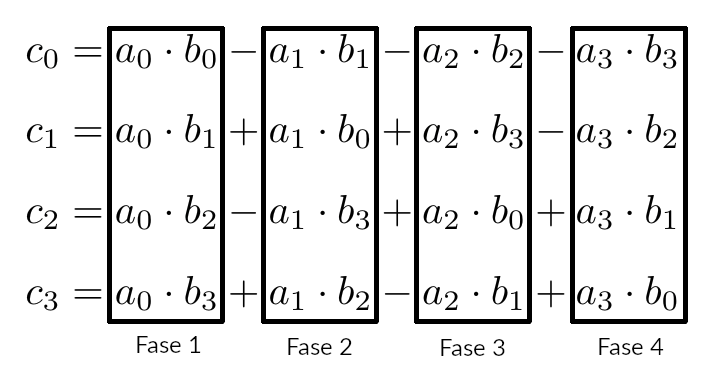
\includegraphics[width=0.4\textwidth]{fases.png}
        \caption{Fases para la multiplicación de cuaterniones.}
        \label{fasesMult}
    \end{figure}
    
Esta separación permite paralelizar la multiplicación, y además efectuarla de modo eficiente, debido a que en todas las fases, el cuaternión $b$ se encuentra completo, pero con sus términos intercambiados de orden. A mayores, por otro lado, en cada Fase aparece un único término del cuaternión $a$, de forma que en la Fase \textit{i} aparece el valor $a_{i}$. A mayores, al principio del cómputo se inicializará un vector con sus valores a 0, que será de utilidad para siguientes cálculos.

La librería \texttt{pmmintrin.h} aporta una operación para hacer un \textit{shuffle} entre los elementos del vector, \texttt{\_mm\_shuffle}, pudiendo obtener así vectores auxiliares para realizar estas operaciones, tal y como aparece en el primer bucle del código. De esta forma, sería necesario realizar cuatro \textit{shuffles} para obtener todos los vectores auxiliares del cuaternión $a$ y otros cuatro para los de $b$, dando un total de 8 ciclos por el momento. De esta forma, se pueden realizar las operaciones entre los vectores auxiliares calculados de $a$ y de $b$ con la operación \texttt{\_mm\_mul\_ps}, la cual tarda un total de 5 ciclos en el procesador en que se ejecutarán las pruebas. Como hay que realizar una única multiplicación por fase, se obtendría un total de 20 ciclos.

A continuación, es necesario realizar las sumas y restas correspondientes para unir las cuatro fases en un único valor. Esto podría realizarse mediante las operaciones \texttt{\_mm\_add\_ps} y \texttt{\_mm\_sub\_ps}, durando cada una 3 ciclos, pero la operación se realiza de término a término, no pudiendo cambiar los signos. La única forma que habría para realizar esto sería utilizar un vector auxiliar con los coeficientes, como $(-1, 1, -1, 1)$, y multiplicarlo por el vector que se quiere añadir, en este caso $(a_{1}\cdot b_{1}, a_{1}\cdot b_{0}, a_{1}\cdot b_{3}, a_{1}\cdot b_{2})$. El problema de esta solución es que implicaría demasiados ciclos, debido a que se tendrían que realizar tres multiplicaciones, cargar el vector auxiliar en memoria, además de diversos \textit{shuffles}.

En el código propuesto se ha abordado una solución más eficiente utilizando la función \texttt{\_mm\_addsub\_ps}, la cual realiza una mezcla entre una suma y una resta, de forma que resta los términos impares y suma los pares. Esta operación, de 3 ciclos en el procesador de las pruebas, resulta muy útil en el problema a abordar debido a que en todas las fases será necesario restar dos términos y sumar otros dos. De esta forma, en la primera fase se puede realizar la operación \texttt{addsub} sin necesidad de realizar cómputos adicionales, pero en las dos últimas fases será necesario reorganizar los vectores con \texttt{\_mm\_shuffle} para poder utilizar el \texttt{addsub} correctamente. Por lo tanto, como se realizan tres \texttt{\_mm\_addsub\_ps} y son necesarios dos shuffles para adaptar los vectores auxiliares de la Fase 3 y Fase 4, dos \textit{shuffles} para ajustar el vector resultante al realizar los \texttt{addsub} y uno último para recolocarlo de forma correcta, se obtienen así un total de 13 ciclos; junto los 28 anteriores, se realizaría esta parte en un total de \textit{41 ciclos}.

Por otro lado, este número puede ser reducido en dos ciclos más si, en vez de reajustar los vectores auxiliares después de la multiplicación, se ajustan ya en el momento del \textit{shuffle} del cuaternión $b$. Esto no afectará en ningún momento al resultado final debido a que todos los términos se multiplican siempre por el mismo valor del cuaternión $a$, teniendo que gestionar así simplemente los tres \textit{shuffles} del vector resultante y obteniendo una multiplicación de cuaterniones en \textit{39 ciclos}.

El problema podría finalizar aquí, debido a que al haber obtenido una forma de multiplicar cuaterniones vectorialmente, en el siguiente bucle de ejecución sería abordar el problema de la misma forma. Sin embargo, al estar basado este programa en el secuencial optimizado, se ha decidido aprovechar también la característica mostrada en la Ecuación \ref{productoCuatIguales2} sobre la multiplicación de un cuaternión por sí mismo.

En esta ocasión, no se realizarán cómputos por fases debido a que cada término del cuaternión ahora es un único sumando, exceptuando el primero. Como en el segundo, tercer y cuarto término aparece el producto $2\cdot a_{0}\cdot a_{i}$, ahora se obtendrán estos tres valores de forma paralela. Esto se consigue haciendo un \textit{shuffle} del cuaternión $a$, generando un vector que tenga de componentes el primer término del cuaternión. Ahora, con este vector auxiliar de $a$, para obtener el doble se suma con sí mismo. De esta forma se obtiene un nuevo vector $(2\cdot a_{0}, 2\cdot a_{0}, 2\cdot a_{0}, 2\cdot a_{0})$. Hasta ahora se han utilizado un shuffle y un \texttt{\_mm\_add\_ps}, dando un total de 4 ciclos.

El siguiente paso será obtener la multiplicación restante para obtener $2\cdot a_{0}\cdot a_{i}$. Para ello, se multiplica el vector auxiliar por el cuaternión $a$, obteniendo de esta forma el siguiente vector: $(2\cdot a_{0}\cdot a_{0}, 2\cdot a_{0}\cdot a_{1}, 2\cdot a_{0}\cdot a_{2}, 2\cdot a_{0}\cdot a_{3})$. Hasta ahora con la multiplicación adicional se obtiene un total de 9 ciclos. Este último vector calculado se nombrará \texttt{qAux}, ya que se utilizará posteriormente.

Las tres últimas componentes del resultado del cuaternión ya se han obtenido; ahora resta ajustar la primera, lo cual puede suponer un cómputo adicional bastante grande, debido a que es necesario realizar diversas operaciones como multiplicaciones. En este proceso, después de plantearse diversos métodos, ha prevalecido aquel más eficiente de todos los hallados, dispuesto a continuación.

Inicialmente, se calcula con \texttt{\_mm\_mul\_ps} el producto del vector $a$ consigo mismo, dando lugar al vector: $(a_{0}\cdot a_{0}, a_{1}\cdot a_{1}, a_{2}\cdot a_{2}, a_{3}\cdot a_{3})$. Ahora, será necesario restar los valores de las tres últimas componentes a la primera; pero, en vez de realizar diversos shuffles y restas, se ha optado por una operación nueva \texttt{\_mm\_hadd\_ps}, la cual realiza una suma horizontal de los vectores indicados con una duración de 5 ciclos. Con esto se obtiene el siguiente vector: $(a_{0}\cdot a_{0}+a_{1}\cdot a_{1}, a_{2}\cdot a_{2}+a_{3}\cdot a_{3}, a_{0}\cdot a_{0}+a_{1}\cdot a_{1}, a_{2}\cdot a_{2}+a_{3}\cdot a_{3})$.

Lo importante de este último cómputo son los dos primeros términos, los cuales deberán ser restados al primero de \textit{qAux}. Por lo tanto se realiza un \textit{shuffle} con el vector de ceros que se inicializó al comienzo de la computación, obteniendo lo siguiente: $(a_{0}\cdot a_{0}+a_{1}\cdot a_{1}, a_{2}\cdot a_{2}+a_{3}\cdot a_{3}, 0, 0)$.

Posteriormente, se obtiene la primera operación a restar, el vector \textit{qAux} menos $(a_{0}\cdot a_{0}+a_{1}\cdot a_{1}, 0, 0, 0)$, el cual se obtiene mediante un \textit{shuffle} consigo mismo. Si esto se repite con la segunda componente del vector calculado en la anterior operación, se obtendría el resultado final.

De esta forma se realiza el cálculo de una multiplicación de dos cuaterniones iguales en \textit{28 ciclos}, un número bastante inferior a los \textit{39} ciclos de una multiplicación normal.

\begin{lstlisting}[style=CStyle, title=Código con la multiplicación vectorizada.]
#include <stdio.h>
#include <stdlib.h>
#include <math.h>
#include <time.h>
#include <unistd.h>
#include <pmmintrin.h>


/* Características de la CPU */

// Múltiplo del que tienen que ser las direcciones de
// memoria a reservar para un alineado correcto para SIMD
#define ALIN_MULT 16

/* Macros varias */
#define FALSE 0
#define TRUE 1


/* Prototipos de las funciones a emplear */
void inicializarVectorCuaternion( float **vector, size_t
    numElementos, int valoresAleatorios );
void liberarVectorCuaternion( float **vector );


/* Main */

int main(int argc, char **argv)
{
    /* Variables a emplear */

    // Número de cuaterniones contenidos en cada array
    size_t n;

    // Orden de magnitud del tamaño de los vectores de
    // input
    size_t q;

    // Vectores de cuaterniones de valores aleatorios
    // (input)
    float *a;
    float *b;

    // Vector auxiliar de cuaterniones
    float *c;

    // Cuaternión sobre el que realizar la computación
    // (output)
    float dp[ 4 ];

    // Variable sobre la que contabilizar el tiempo
    // transcurrido
    double ck;

    // Contadores
    int i;

    // Variable auxiliar para indicar el cuaternión "a"
    // actual
    __m128 qA;

    // Variable auxiliar para indicar el cuaternión "b"
    // actual
    __m128 qB;

    // Variable auxiliar para almacenar el resultado del
    // producto de los cuaterniones qA * qB
    __m128 qC;

    // Cuaternión final sobre el que se realiza el cómputo
    __m128 qDP;

    // Cuaterniones auxiliares para la realización del
    // producto
    __m128 qA0;
    __m128 qA1;
    __m128 qA2;
    __m128 qA3;

    // Cuaternión a 0
    __m128 q0;

    // Cuaternión auxiliar para guardar valores intermedios
    // de una suma
    __m128 qSUM;

    // Cuaternión auxiliar para guardar valores intermedios
    // de la multiplación
    __m128 qMULT;


    /***** Argumentos *****/

    if( argc < 2 )
    {
        printf( "Número de valores incorrecto. Uso: %s "
            "<q>\n", argv[ 0 ] );
        exit( EXIT_FAILURE );
    }

    // Se obtiene el valor de 'q' dado
    q = atoi( argv[ 1 ] );

    if( q <= 0 )
    {
        printf( "El valor de q debe ser mayor que 0\n" );
        exit( EXIT_FAILURE );
    }


    /***** Inicialización *****/

    // Se obtiene una semilla para la generación de números
    // aleatorios
    srand( ( unsigned )time( NULL ) );

    // Se calcula el tamaño final de los vectores de input
    n = ( int )pow( 10, q );

    // Se inicializan los vectores de cuaterniones
    inicializarVectorCuaternion( &a, n, TRUE );
    inicializarVectorCuaternion( &b, n, TRUE );
    inicializarVectorCuaternion( &c, n, FALSE );


    /***** Computación *****/

    // Se inicia el medidor de tiempo
    ck = 0;
    qDP = _mm_setzero_ps();
    q0 = _mm_setzero_ps();
    start_counter();

    // Se almacena en el vector 'c' la multiplicación de
    // los vectores 'a' y 'b'
    for( i = 0; i < n; i++ )
    {
        qA = _mm_load_ps(a + i * 4);
        qB = _mm_load_ps(b + i * 4);

        qA0 = _mm_shuffle_ps(qA, qA, _MM_SHUFFLE(0,0,0,0));
        qA1 = _mm_shuffle_ps(qA, qA, _MM_SHUFFLE(1,1,1,1));
        qA2 = _mm_shuffle_ps(qA, qA, _MM_SHUFFLE(2,2,2,2));
        qA3 = _mm_shuffle_ps(qA, qA, _MM_SHUFFLE(3,3,3,3));

        qC = _mm_mul_ps(qA0, qB);
        qC = _mm_addsub_ps(qC, _mm_mul_ps(qA1,
            _mm_shuffle_ps(qB, qB,
            _MM_SHUFFLE(2, 3, 0, 1))));

        // Se realiza el intercambio de los elementos con
        // signo más y menos para poder realizar el addsub
        qC = _mm_shuffle_ps(qC, qC,
            _MM_SHUFFLE(2, 3, 1, 0));

        qC = _mm_addsub_ps(qC, _mm_mul_ps(qA2,
            _mm_shuffle_ps(qB, qB,
            _MM_SHUFFLE(0, 1, 3, 2))));

        qC = _mm_shuffle_ps(qC, qC,
            _MM_SHUFFLE(2, 1, 3, 0));
        qC = _mm_addsub_ps(qC, _mm_mul_ps(qA3,
            _mm_shuffle_ps(qB, qB,
            _MM_SHUFFLE(0, 2, 1, 3))));

        // Recolocación del cuaternión qC
        qC = _mm_shuffle_ps(qC, qC,
            _MM_SHUFFLE(3, 1, 2, 0));
    }

    // Se inicializan los valores del cuaternión 'dp' a '0'

    // Se realiza sobre el cuaternión 'dp' la suma de la
    // multiplicación de cada cuaternión del vector 'c' por
    // sí mismo
    for( i = 0; i < n; i++ )
    {
        // Se guardan las componentes del cuaternión
        // iterado
        qA0 = _mm_shuffle_ps(qC, qC,
            _MM_SHUFFLE(0, 0, 0, 0));

        // Se realiza la suma de a + a
        qSUM = _mm_add_ps(qC, qC);

        // Se obtiene el cuaternion (2a0*a0, 2a0*a1,
        // 2a0*a2, 2a0*a3)
        qMULT = _mm_mul_ps(qSUM, qA0);

        // Se obtiene el productor de a * a
        qA1 = _mm_mul_ps(qC, qC);

        // Se obtiene (a0a0+a1a1, a2a2+a3a3, a0a0+a1a1,
        // a2a2+a3a3)
        qSUM = _mm_hadd_ps(qA1, qA1);

        // Se obtiene (a0a0+a1a1, a2a2+a3a3, 0, 0)
        qSUM = _mm_shuffle_ps(qSUM, q0,
            _MM_SHUFFLE(3,2,1,0));

        // Se obtiene (a0a0+a1a1, 0, 0, 0)
        qA1 = _mm_shuffle_ps(qSUM, q0,
            _MM_SHUFFLE(0,0,2,0));

        // Se realiza la resta sobre qMULT
        qMULT = _mm_sub_ps(qMULT, qA1);

        // Se obtiene (a2a2+a3a3, 0, 0, 0)
        qA1 = _mm_shuffle_ps(qSUM, q0,
            _MM_SHUFFLE(0,0,2,1));

        // Se resta
        qMULT = _mm_sub_ps(qMULT, qA1);

        // Se le añade al cuaternion suma
        qDP = _mm_add_ps(qDP, qMULT);
    }

    _mm_store_ps(dp, qDP);

    // Se finaliza el medidor de tiempo
    ck = get_counter();

    printf( "%d,%lu,%1.10lf\n", atoi( argv[ 2 ] ), q, ck );
    
    printf( "Resultado: [%f, %f, %f, %f]\n", dp[ 0 ],
        dp[ 1 ], dp[ 2 ], dp[ 3 ] );

    // Se libera la memoria reservada
    liberarVectorCuaternion( &a );
    liberarVectorCuaternion( &b );
    liberarVectorCuaternion( &c );


    return( EXIT_SUCCESS );
}


void inicializarVectorCuaternion( float **vector, size_t
    numElementos, int valoresAleatorios )
{
    // Contador
    int i;


    // Se reserva la memoria necesaria para el vector de
    // cuaterniones
    if( ( *vector = _mm_malloc( numElementos * 4 *
        sizeof( float ), ALIN_MULT ) ) == NULL )
    {
        perror( "Reserva de memoria del vector de "
            "cuaterniones fallida" );
        exit( EXIT_FAILURE );
    }

    if( valoresAleatorios == TRUE )
    {
        // Y se genera en cada posición de los cuaterniones
        // de los vectores un valor entre 1 y 2
        for( i = 0; i < numElementos; i++ )
        {
            *( *vector + i * 4 ) = ( ( double )rand() /
                RAND_MAX + 1 ) * pow( -1, rand() % 2 );
            *( *vector + i * 4 + 1 ) = ( ( double )rand() /
                RAND_MAX + 1 ) * pow( -1, rand() % 2 );
            *( *vector + i * 4 + 2 ) = ( ( double )rand() /
                RAND_MAX + 1 ) * pow( -1, rand() % 2 );
            *( *vector + i * 4 + 3 ) = ( ( double )rand() /
                RAND_MAX + 1 ) * pow( -1, rand() % 2 );
        }
    }

    else
    {
        // En caso contrario, se inicializan los valores a '0'
        for( i = 0; i < numElementos; i++ )
        {
            *( *vector + i * 4 ) = 0;
            *( *vector + i * 4 + 1 ) = 0;
            *( *vector + i * 4 + 2 ) = 0;
            *( *vector + i * 4 + 3 ) = 0;
        }
    }
}


void liberarVectorCuaternion( float **vector )
{
    _mm_free( *vector );
}
\end{lstlisting}

Una vez vista la alternativa de vectorizar la multiplicación de dos cuaterniones, la otra opción consiste simplemente en vectorizar los bucles de la computación. Es decir, dado que un cuaternión puede almacenar un total de cuatro elementos de punto flotante, es posible tomar partido de dicha característica para, en cada iteración de los bucles, realizar las operaciones del código secuencial optimizado sobre cuatro parejas de cuaterniones, en lugar de sobre una única pareja.

El código resultado de esta técnica de vectorización del programa puede verse a continuación.

\begin{lstlisting}[style=CStyle, title=Código con la ejecución del bucle vectorizada.]
#include <stdio.h>
#include <stdlib.h>
#include <math.h>
#include <time.h>
#include <unistd.h>
#include <pmmintrin.h>


// Múltiplo del que tienen que ser las direcciones de
// memoria a reservar para un alineado correcto para SIMD
#define ALIN_MULT 16


/* Macros varias */
#define FALSE 0
#define TRUE 1


/* Estructura en la que almacenar un vector de
   cuaterniones */
struct VectorCuaterniones
{
    float *w;
    float *x;
    float *y;
    float *z;
};


/* Prototipos de las funciones a emplear */
void inicializarVectorCuaternion( struct VectorCuaterniones
    *vector, size_t numElementos, int valoresAleatorios );
void liberarVectorCuaternion( struct VectorCuaterniones
    *vector );


/* Main */

int main(int argc, char **argv)
{
    /* Variables a emplear */

    // Número de cuaterniones contenidos en cada array
    size_t n;

    // Orden de magnitud del tamaño de los vectores de
    // input
    size_t q;

    // Vectores de cuaterniones de valores aleatorios
    // (input)
    struct VectorCuaterniones a;
    struct VectorCuaterniones b;

    // Vector auxiliar de cuaterniones
    struct VectorCuaterniones c;

    // Cuaternión sobre el que realizar la computación
    // (output)
    float dp[ 4 ];

    // Cuaterniones sobre los que almacenar temporalmente
    // los resultados del segundo bucle en lugar de
    // efecutar constantemente reducciones
    __m128 dp0, dp1, dp2, dp3;

    // Variable sobre la que contabilizar el tiempo
    // transcurrido
    double ck;

    // Variables auxiliares en las que almacenar elementos
    // de cuaterniones
    __m128 a0, a1, a2, a3, b0, b1, b2, b3, c0, c1, c2, c3;

    // Contadores
    int i;


    /***** Argumentos *****/

    if( argc < 2 )
    {
        printf( "Número de valores incorrecto. Uso: %s "
            "<q>\n", argv[ 0 ] );
        exit( EXIT_FAILURE );
    }

    // Se obtiene el valor de 'q' dado
    q = atoi( argv[ 1 ] );

    if( q <= 0 )
    {
        printf( "El valor de q debe ser mayor que 0\n" );
        exit( EXIT_FAILURE );
    }


    /***** Inicialización *****/

    // Se obtiene una semilla para la generación de números
    // aleatorios
    srand( ( unsigned )time( NULL ) );

    // Se calcula el tamaño final de los vectores de input
    n = ( int )pow( 10, q );

    // Se inicializan los vectores de cuaterniones
    inicializarVectorCuaternion( &a, n, TRUE );
    inicializarVectorCuaternion( &b, n, TRUE );
    inicializarVectorCuaternion( &c, n, FALSE );


    /***** Computación *****/

    // Se inicia el medidor de tiempo
    ck = 0;
    start_counter();

    // Se almacena en el vector 'c' la multiplicación de
    // los vectores 'a' y 'b'; en cada iteración del bucle
    // se computan 4 multiplicaciones de cuaterniones
    for( i = 0; i < n; i += 4 )
    {
        // Se guardan las componentes de los cuatro
        // cuaterniones iterados en cada vector
        a0 = _mm_load_ps( a.w + i );
        a1 = _mm_load_ps( a.x + i );
        a2 = _mm_load_ps( a.y + i );
        a3 = _mm_load_ps( a.z + i );

        b0 = _mm_load_ps( b.w + i );
        b1 = _mm_load_ps( b.x + i );
        b2 = _mm_load_ps( b.y + i );
        b3 = _mm_load_ps( b.z + i );

        // Se realiza el producto de los cuatro primeros
        // cuaterniones por los cuatro del vector 'b'
        c0 = _mm_sub_ps( _mm_sub_ps( _mm_sub_ps(
            _mm_mul_ps( a0, b0 ), _mm_mul_ps( a1, b1 ) ),
            _mm_mul_ps( a2, b2 ) ), _mm_mul_ps( a3, b3 ) );
            
        c1 = _mm_sub_ps( _mm_add_ps( _mm_add_ps(
            _mm_mul_ps( a0, b1 ), _mm_mul_ps( a1, b0 ) ),
            _mm_mul_ps( a2, b3 ) ), _mm_mul_ps( a3, b2 ) );
            
        c2 = _mm_add_ps( _mm_add_ps( _mm_sub_ps(
            _mm_mul_ps( a0, b2 ), _mm_mul_ps( a1, b3 ) ),
            _mm_mul_ps( a2, b0 ) ), _mm_mul_ps( a3, b1 ) );
            
        c3 = _mm_add_ps( _mm_sub_ps( _mm_add_ps(
            _mm_mul_ps( a0, b3 ), _mm_mul_ps( a1, b2 ) ),
            _mm_mul_ps( a2, b1 ) ), _mm_mul_ps( a3, b0 ) );

        /* Referencia

        *( c + i * 4 ) = a0 * b0 - a1 * b1 - a2 * b2 - a3 *
            b3;
        *( c + i * 4 + 1 ) = a0 * b1 + a1 * b0 + a2 * b3 -
            a3 * b2;
        *( c + i * 4 + 2 ) = a0 * b2 - a1 * b3 + a2 * b0 +
            a3 * b1;
        *( c + i * 4 + 3 ) = a0 * b3 + a1 * b2 - a2 * b1 +
            a3 * b0; */

        // Se extraen los valores de los cuatro
        // cuaterniones resultado componente a componente y
        // se almacenan en el vector 'c'

        // Componente 'w'
        _mm_store_ps( c.w + i, c0 );

        // Componente 'x'
        _mm_store_ps( c.x + i, c1 );

        // Componente 'y'
        _mm_store_ps( c.y + i, c2 );

        // Componente 'z'
        _mm_store_ps( c.z + i, c3 );
    }

    // Se inicializan a (0, 0, 0, 0) los cuaterniones
    // auxiliares para este bucle
    dp0 = _mm_setzero_ps();
    dp1 = _mm_setzero_ps();
    dp2 = _mm_setzero_ps();
    dp3 = _mm_setzero_ps();

    // Se realiza sobre el cuaternión 'dp' la suma de la
    // multiplicación de cada cuaternión del vector 'c' por
    // sí mismo
    for( i = 0; i < n; i += 4 )
    {
        // Se guardan las componentes de los cuatro
        // cuaterniones iterados en el vector 'c'
        a0 = _mm_load_ps( c.w + i );
        a1 = _mm_load_ps( c.x + i );
        a2 = _mm_load_ps( c.y + i );
        a3 = _mm_load_ps( c.z + i );

        // Se realiza el producto de los cuatro primeros
        // cuaterniones por sí mismos
        c0 = _mm_sub_ps( _mm_sub_ps( _mm_sub_ps(
            _mm_mul_ps( a0, a0 ), _mm_mul_ps( a1, a1 ) ),
            _mm_mul_ps( a2, a2 ) ), _mm_mul_ps( a3, a3 ) );
        c1 = _mm_mul_ps( _mm_add_ps( a0, a0 ), a1 );
        c2 = _mm_mul_ps( _mm_add_ps( a0, a0 ), a2 );
        c3 = _mm_mul_ps( _mm_add_ps( a0, a0 ), a3 );

        /* Referencia

        dp[ 0 ] += c0 * c0 - c1 * c1 - c2 * c2 - c3 * c3;
        dp[ 1 ] += ( c0 + c0 ) * c1;
        dp[ 2 ] += ( c0 + c0 ) * c2;
        dp[ 3 ] += ( c0 + c0 ) * c3; */

        // Se añaden los 4 valores calculados para cada
        // componente i a la variable auxiliar del
        // componente i
        dp0 = _mm_add_ps( dp0, c0 );
        dp1 = _mm_add_ps( dp1, c1 );
        dp2 = _mm_add_ps( dp2, c2 );
        dp3 = _mm_add_ps( dp3, c3 );
    }

    // Se extraen los valores de los cuaterniones 
    // auxiliares componente a componente y se guardan en
    // las componentes del cuaternión 'dp'

    // Componente 'w'
    dp[ 0 ] = _mm_cvtss_f32( _mm_hadd_ps( _mm_hadd_ps( dp0,
        dp0 ), dp0 ) );

    // Componente 'x'
    dp[ 1 ] = _mm_cvtss_f32( _mm_hadd_ps( _mm_hadd_ps( dp1,
        dp1 ), dp1 ) );

    // Componente 'y'
    dp[ 2 ] = _mm_cvtss_f32( _mm_hadd_ps( _mm_hadd_ps( dp2,
        dp2 ), dp2 ) );

    // Componente 'z'
    dp[ 3 ] = _mm_cvtss_f32( _mm_hadd_ps( _mm_hadd_ps( dp3,
        dp3 ), dp3 ) );

    // Se finaliza el medidor de tiempo
    ck = get_counter();

    printf( "%d,%lu,%1.10lf\n", atoi( argv[ 2 ] ), q, ck );
    
    printf( "Resultado: [%f, %f, %f, %f]\n", dp[ 0 ],
        dp[ 1 ], dp[ 2 ], dp[ 3 ] );

    // Se libera la memoria reservada
    liberarVectorCuaternion( &a );
    liberarVectorCuaternion( &b );
    liberarVectorCuaternion( &c );


    return( EXIT_SUCCESS );
}


void inicializarVectorCuaternion( struct VectorCuaterniones
    *vector, size_t numElementos, int valoresAleatorios )
{
    // Contador
    int i;


    // Se reserva la memoria necesaria para el vector de
    // cuaterniones
    if( ( vector->w = _mm_malloc( numElementos *
        sizeof( float ), ALIN_MULT ) ) == NULL )
    {
        perror( "Reserva de memoria del vector de "
            "cuaterniones (componente 'w') fallida" );
        exit( EXIT_FAILURE );
    }

    if( ( vector->x = _mm_malloc( numElementos *
        sizeof( float ), ALIN_MULT ) ) == NULL )
    {
        perror( "Reserva de memoria del vector de "
            "cuaterniones (componente 'x') fallida" );
        exit( EXIT_FAILURE );
    }

    if( ( vector->y = _mm_malloc( numElementos *
        sizeof( float ), ALIN_MULT ) ) == NULL )
    {
        perror( "Reserva de memoria del vector de "
            "cuaterniones (componente 'y') fallida" );
        exit( EXIT_FAILURE );
    }

    if( ( vector->z = _mm_malloc( numElementos *
        sizeof( float ), ALIN_MULT ) ) == NULL )
    {
        perror( "Reserva de memoria del vector de "
            "cuaterniones (componente 'z') fallida" );
        exit( EXIT_FAILURE );
    }

    if( valoresAleatorios == TRUE )
    {
        // Y se genera en cada posición de los cuaterniones
        // de los vectores un valor entre 1 y 2
        for( i = 0; i < numElementos; i++ )
        {
            *( vector->w + i ) = ( ( double )rand() /
                RAND_MAX + 1 ) * pow( -1, rand() % 2 );
            *( vector->x + i ) = ( ( double )rand() /
                RAND_MAX + 1 ) * pow( -1, rand() % 2 );
            *( vector->y + i ) = ( ( double )rand() /
                RAND_MAX + 1 ) * pow( -1, rand() % 2 );
            *( vector->z + i ) = ( ( double )rand() /
                RAND_MAX + 1 ) * pow( -1, rand() % 2 );
        }
    }

    else
    {
        // En caso contrario, se inicializan los valores a 
        // '0'
        for( i = 0; i < numElementos; i++ )
        {
            *( vector->w + i ) = 0;
            *( vector->x + i ) = 0;
            *( vector->y + i ) = 0;
            *( vector->z + i ) = 0;
        }
    }
}


void liberarVectorCuaternion( struct VectorCuaterniones
    *vector )
{
    _mm_free( vector->w );
    _mm_free( vector->x );
    _mm_free( vector->y );
    _mm_free( vector->z );
}
\end{lstlisting}

Tal y como se ha comentado, la adaptación de los bucles del cómputo para ser vectorizados ha consistido, de forma general, en un sencillo procedimiento de tomar los elementos del lenguaje C para un dato de punto flotante, y sustituirlas por sus contrapartes en instrucciones SSE para vectores de cuatro elementos de punto flotante. Para ello:
\begin{itemize}
    \item Las variables auxiliares empleadas en los bucles pasan a ser ahora de tipo \texttt{\_\_m128} en lugar de \texttt{float}.
    \item Las operaciones \texttt{+}, \texttt{-} y \texttt{*} son sustituidas por \texttt{\_mm\_add\_ps()}, \texttt{\_mm\_sub\_ps()} y \texttt{\_mm\_mul\_ps()} respectivamente.
\end{itemize}

Para la carga y escritura de los valores de los cuaterniones en memoria, se ha decidido modificar además la disposición de los datos en memoria: ahora, un vector de cuaterniones se compone a su vez de otros cuatro vectores, y las componentes de un cuaternión del vector no se disponen de forma contigua, si no que cada una de ellas se almacena en su correspondiente vector. Esta necesidad surge como consecuencia de que ahora cada variable auxiliar contenga el mismo término pero de cuatro cuaterniones diferentes.

Supóngase una variable auxiliar $aux$ que contiene el primer término de los cuatro cuaterniones del vector $a$ operados en una iteración del primer bucle. Tal y como se estructuraba anteriormente la memoria, los cuatro términos que se deben cargar en $aux$ se encontraban distanciados entre sí dentro del vector $a$; concretamente, entre cada uno de los términos se encontrarían un total de tres datos de punto flotante. Esto supondría una ligera penalización de rendimiento al no leer datos contiguos en memoria, reduciéndose los beneficios del principio localidad; del mismo modo, también surgiría una leve penalización a la hora de almacenar los datos en la memoria del vector $c$, puesto que no se escribirían en posiciones de memoria contiguas.

Por ello, se ha adoptado la nueva estructuración de los datos en memoria de modo que, tal y como refleja el anterior código, las cargas de datos a una variable \texttt{\_\_m128} y las escrituras de ellas a memoria se efectúan sobre posiciones de memoria completamente contiguas, aprovechándose todo lo posible los beneficios del principio de localidad.

Finalmente, cabe destacar que, a lo largo de la ejecución del segundo bucle, no se efectúa directamente la reducción de la multiplicación $c \cdot c$ sobre un único cuaternión. Al multiplicarse en cada iteración del bucle cuatro parejas de cuaterniones, la opción más inmediata sería, para cada componente $i$, sumar los cuatro valores correspondientes a las cuatro multiplicaciones realizadas, y sumar dicho valor al componente $i$ del resultado $dp$.

En lugar de ello, la reducción de las componentes de $c \cdot c$ se efectúa sobre cuatro variables \texttt{\_\_m128} independientes (\texttt{dp0}, \texttt{dp1}, \texttt{dp2} y \texttt{dp3}), de modo que la reducción a computar sobre los valores del elemento $i$ de $c \cdot c$ no se concentra en un único elemento de punto flotante, si no que se distribuye entre los cuatro elementos de la variable \texttt{dp\{i\}}. Esto evita la necesidad de realizar, al final de cada iteración, una reducción de punto flotante sobre los valores de \texttt{dp\{i\}} para ser almacenados en un único elemento de punto flotante, como se propuso previamente. Por lo tanto, tan solo es necesario efectuar, para cada componente de $c \cdot c$, una reducción sobre los valores repartidos entre los cuatro elementos de la variable \texttt{dp\{i\}} tras la finalización del segundo bucle.

La importancia de ello es el considerable ahorro de ciclos del procesador durante el cómputo: en lugar de emplear en cada iteración del bucle, para efectuar la reducción sobre $dp$, un total de ocho instrucciones \texttt{\_mm\_hadd\_ps()} y cuatro instrucciones \texttt{\_mm\_cvtss\_f32()}, se emplean tan solo cuatro instrucciones \texttt{\_mm\_add\_ps()}, sumadas a ocho instrucciones \texttt{\_mm\_hadd\_ps()} y cuatro instrucciones \texttt{\_mm\_cvtss\_f32()} tras la finalización del bucle.

\subsection{Implementación multihilo}

El último código a realizar, basado en la versión secuencial optimizada, se trata de aquel que incorpora la programación multihilo, como se comentó anteriormente.

Se dispone a continuación el código fuente correspondiente. El número de hilos a emplear puede variarse fácilmente modificando una directiva del preprocesador de C; por ello, no se disponen todos los programas correspondientes a una sección, sino que se muestra tan solo uno de ellos ya que las únicas diferencias entre ellos se encontrarían en el valor de dicha directiva.

\begin{lstlisting}[style=CStyle, title=Código multihilo.]
#include <stdio.h>
#include <stdlib.h>
#include <math.h>
#include <time.h>
#include <unistd.h>
#include <pmmintrin.h>
#include <omp.h>


// Múltiplo del que tienen que ser las direcciones de
// memoria a reservar para un alineado correcto para SIMD
#define ALIN_MULT 16

/* Macros varias */
#define FALSE 0
#define TRUE 1
#define NUM_HILOS 16


/* Prototipos de las funciones a emplear */
void inicializarVectorCuaternion( float **vector, size_t
    numElementos, int valoresAleatorios );
void liberarVectorCuaternion( float **vector );


/* Main */

int main(int argc, char **argv)
{
    /* Variables a emplear */

    // Número de cuaterniones contenidos en cada array
    size_t n;

    // Orden de magnitud del tamaño de los vectores de
    // input
    size_t q;

    // Vectores de cuaterniones de valores aleatorios
    // (input)
    float *a;
    float *b;

    // Vector auxiliar de cuaterniones
    float *c;

    // Cuaternión sobre el que realizar la computación
    // (output)
    float dp[ 4 ] = { 0, 0, 0, 0 };

    // Variables auxiliares para efectuar la reducción de
    // punto flotante
    float dpAux[ NUM_HILOS ][ 4 ];
    float dpPriv0, dpPriv1, dpPriv2, dpPriv3;

    // Variable sobre la que contabilizar el tiempo
    // transcurrido
    double ck;

    // Variables auxiliares en las que almacenar elementos
    // de cuaterniones
    float a0, a1, a2, a3, b0, b1, b2, b3, c0, c1, c2, c3;

    // Variable en la que almacenar un número identificador
    // de un hilo
    int numHilo;

    // Contadores
    int i;


    /***** Argumentos *****/

    if( argc < 2 )
    {
        printf( "Número de valores incorrecto. Uso: %s "
            "<q>\n", argv[ 0 ] );
        exit( EXIT_FAILURE );
    }

    // Se obtiene el valor de 'q' dado
    q = atoi( argv[ 1 ] );

    if( q <= 0 )
    {
        printf( "El valor de q debe ser mayor que 0\n" );
        exit( EXIT_FAILURE );
    }


    /***** Inicialización *****/

    // Se obtiene una semilla para la generación de números
    // aleatorios
    srand( ( unsigned )time( NULL ) );

    // Se calcula el tamaño final de los vectores de input
    n = ( int )pow( 10, q );

    // Se inicializan los vectores de cuaterniones
    inicializarVectorCuaternion( &a, n, TRUE );
    inicializarVectorCuaternion( &b, n, TRUE );
    inicializarVectorCuaternion( &c, n, FALSE );


    /***** Computación *****/

    // Se inicia el medidor de tiempo
    ck = 0;
    start_counter();

    // Se almacena en el vector 'c' la multiplicación de
    // los vectores 'a' y 'b'; la realización del bucle se
    // repartirá entre todos los hilos indicados
    #pragma omp parallel private( i, a0, a1, a2, a3, b0,
        b1, b2, b3 ) num_threads( NUM_HILOS )
    {
        #pragma omp for
        for( i = 0; i < n; i++ )
        {
            // Se guardan las componentes de los
            // cuaterniones iterados
            a0 = *( a + i * 4 );
            a1 = *( a + i * 4 + 1 );
            a2 = *( a + i * 4 + 2 );
            a3 = *( a + i * 4 + 3 );

            b0 = *( b + i * 4 );
            b1 = *( b + i * 4 + 1 );
            b2 = *( b + i * 4 + 2 );
            b3 = *( b + i * 4 + 3 );

            // Se realiza el producto del primer cuaternión
            // por el segundo
            *( c + i * 4 ) = a0 * b0 - a1 * b1 - a2 * b2 -
                a3 * b3;
            *( c + i * 4 + 1 ) = a0 * b1 + a1 * b0 + a2 *
                b3 - a3 * b2;
            *( c + i * 4 + 2 ) = a0 * b2 - a1 * b3 + a2 *
                b0 + a3 * b1;
            *( c + i * 4 + 3 ) = a0 * b3 + a1 * b2 - a2 *
                b1 + a3 * b0;
        }
    }

    // Se realiza sobre el cuaternión 'dp' la suma de la
    // multiplicación de cada cuaternión del vector 'c' por
    // sí mismo; la realización del bucle se repartirá
    // entre todos los hilos indicados
    #pragma omp parallel private( numHilo, i, c0, c1, c2,
        c3, dpPriv0, dpPriv1, dpPriv2, dpPriv3 )
        num_threads( NUM_HILOS )
    {
        // Se obtiene el número de hilo
        numHilo = omp_get_thread_num();

        // Se inicializan los valores del contenedor
        // auxiliar a emplear del cuaternión 'dp'
        dpPriv0 = 0;
        dpPriv1 = 0;
        dpPriv2 = 0;
        dpPriv3 = 0;

        #pragma omp for
        for( i = 0; i < n; i++ )
        {
            // Se guardan las componentes del cuaternión
            // iterado
            c0 = *( c + i * 4 );
            c1 = *( c + i * 4 + 1 );
            c2 = *( c + i * 4 + 2 );
            c3 = *( c + i * 4 + 3 );

            // Se realiza el producto del primer cuaternión
            // por el segundo
            dpPriv0 += c0 * c0 - c1 * c1 - c2 * c2 - c3 *
                c3;
            dpPriv1 += ( c0 + c0 ) * c1;
            dpPriv2 += ( c0 + c0 ) * c2;
            dpPriv3 += ( c0 + c0 ) * c3;
        }

        // Se guardan en el contenedor auxiliar los
        // resultados obtenidos
        dpAux[ numHilo ][ 0 ] = dpPriv0;
        dpAux[ numHilo ][ 1 ] = dpPriv1;
        dpAux[ numHilo ][ 2 ] = dpPriv2;
        dpAux[ numHilo ][ 3 ] = dpPriv3;
    }

    // Finalmente, el hilo máster reúne los resultados
    // obtenidos por cada hilo
    for( i = 0; i < NUM_HILOS; i++ )
    {
        dp[ 0 ] += dpAux[ i ][ 0 ];
        dp[ 1 ] += dpAux[ i ][ 1 ];
        dp[ 2 ] += dpAux[ i ][ 2 ];
        dp[ 3 ] += dpAux[ i ][ 3 ];
    }

    // Se finaliza el medidor de tiempo
    ck = get_counter();

    printf( "%d,%lu,%1.10lf\n", atoi( argv[ 2 ] ), q, ck );
    
    printf( "Resultado: [%f, %f, %f, %f]\n", dp[ 0 ],
        dp[ 1 ], dp[ 2 ], dp[ 3 ] );

    // Se libera la memoria reservada
    liberarVectorCuaternion( &a );
    liberarVectorCuaternion( &b );
    liberarVectorCuaternion( &c );


    return( EXIT_SUCCESS );
}


void inicializarVectorCuaternion( float **vector, size_t
    numElementos, int valoresAleatorios )
{
    // Contador
    int i;


    // Se reserva la memoria necesaria para el vector de
    // cuaterniones
    if( ( *vector = _mm_malloc( numElementos * 4 *
        sizeof( float ), ALIN_MULT ) ) == NULL )
    {
        perror( "Reserva de memoria del vector de "
            "cuaterniones fallida" );
        exit( EXIT_FAILURE );
    }

    if( valoresAleatorios == TRUE )
    {
        // Y se genera en cada posición de los cuaterniones
        // de los vectores un valor entre 1 y 2
        for( i = 0; i < numElementos; i++ )
        {
            *( *vector + i * 4 ) = ( ( double )rand() /
                RAND_MAX + 1 ) * pow( -1, rand() % 2 );
            *( *vector + i * 4 + 1 ) = ( ( double )rand() /
                RAND_MAX + 1 ) * pow( -1, rand() % 2 );
            *( *vector + i * 4 + 2 ) = ( ( double )rand() /
                RAND_MAX + 1 ) * pow( -1, rand() % 2 );
            *( *vector + i * 4 + 3 ) = ( ( double )rand() /
                RAND_MAX + 1 ) * pow( -1, rand() % 2 );
        }
    }

    else
    {
        // En caso contrario, se inicializan los valores a '0'
        for( i = 0; i < numElementos; i++ )
        {
            *( *vector + i * 4 ) = 0;
            *( *vector + i * 4 + 1 ) = 0;
            *( *vector + i * 4 + 2 ) = 0;
            *( *vector + i * 4 + 3 ) = 0;
        }
    }
}


void liberarVectorCuaternion( float **vector )
{
    _mm_free( *vector );
}
\end{lstlisting}

Como se puede observar, la adaptación del código para el empleo de una cantidad arbitraria de hilos que colaboren en la realización del bucle computacional es, en primera instancia, un procedimiento sencillo. Una ejecución que se pretende paralelizar (una por cada bucles) debe contenerse dentro de un único bloque empleando llaves, y esta región debe ser encabezada por la directiva \texttt{\#pragma omp parallel}, indicándose el número de hilos que se ejecutarán a lo largo de dicho bloque, y especificando qué variables no serán compartidas entre los hilos. Por otra parte, para repartir la realización de un bucle contenido en un bloque entre los hilos presentes en dicho bloque, tan solo es necesario añadir la directiva \texttt{\#pragma omp for} para que las iteraciones de bucle sean repartidas automáticamente entre todos los hilos disponibles.

Tocante a las variables que se especifican como privadas para cada hilo, puede observarse que es necesario incluir en cada bucle el contador \texttt{i} y todas aquellas variables auxiliares en las que se almacenan los datos empleados como operandos en una iteración, como consecuencia de que, en un momento dado, cada hilo se encuentre ejecutando una iteración diferente del bucle.

Además, cabe destacar que, en el segundo bucle, se emplea ahora una serie de variables auxiliares: \texttt{dpPriv0}, \texttt{dpPriv1}, \texttt{dpPriv2} y \texttt{dpPriv3}. Estas variables son empleadas por cada hilo de forma privada, de modo que la reducción que cada hilo realiza sobre la operación $c \cdot c$ no se concentra en todo momento sobre $dp$, sino que se distribuye entre dichas variables privadas. Cuando un hilo finaliza, almacena su cómputo en un vector auxiliar \texttt{dpAux} en el que se concentrarán todas las reducciones de todos los hilos, y será el hilo principal quien se encargue de combinar los valores de dicho vector para obtener el resultado final de $dp$.

El motivo por el cual se ha tomado la decisión es que, al forzar a cada hilo a efectuar la reducción de $c \cdot c$ sobre una variable privada, y acceder tan solo a una variable compartida \texttt{dpAux} al finalizar todas las iteraciones que le correspondan, se obtiene un aumento significativo del rendimiento al deshacerse de mecanismos de control de acceso a una variable compartida. Para ello, debe tenerse presente que, cuando existen varios hilos en ejecución y tratan de acceder a una variable compartida, OpenMP se encarga de implementar los mecanismos de control de carreras críticas necesarios para emplear dicha variable de un modo correcto. Por lo tanto, si los hilos operasen directamente sobre $dp$, se estarían activando y desactivando constantemente mecanismos de control para poder acceder a $dp$, suponiendo un \textit{overhead} notable en el tiempo de computación.

En el primer bucle no se ha tomado la decisión de que cada uno de los hilos compute los valores que le correspondan de $c$ sobre un vector privado, en lugar de hacerlo sobre $c$ directamente, a pesar de que cada posición de $c$ tan solo sea escrita por un hilo y OpenMP decida incorporar de todos modos mecanismos de control de acceso. El motivo de ello es que, si cada hilo calculase parte de $c$ sobre un vector auxiliar, antes de finalizar debería copiar todos los valores generados a sus correspondientes posiciones de $c$, lo cual sería un procedimiento lento sin duda alguna, y además también se estarían activando y desactivando constantemente mecanismos de control de acceso a $c$ porque es muy probable que la mayor parte de los hilos decidan trasladar sus valores a $c$ al mismo tiempo.

\section{Análisis de las implementaciones vectorizadas con IACA}\label{IACA}

\subsection{Funcionamiento de IACA}

En la Sección \ref{descripcionComputador} se destacó que se emplearía la herramienta Intel Architecture Code Analyzer (IACA). Esta utilidad permite analizar un código ensamblador dado para \textbf{estimar} su rendimiento sobre una CPU específica, además de ayudar en la detección de posibles cuellos de botellas creados como consecuencia de una mala praxis en el proceso de programación. Para ello, efectúa un análisis estático de dependencias de datos, \textit{throughput} y latencia del código.

La utilidad de esta herramienta en estos experimentos surge directamente de haber concretado la CPU sobre la cual se ejecutarán todas las pruebas. Por ello, es posible realizar un análisis previo sobre los programas vectorizados, excluyendo los demás de estos análisis, dado que los autores de este informe no se encontraban familiarizados con la programación vectorial antes de la realización de los programas mostrados anteriormente. 

Para ello, los programas son compilados empleando la utilidad ICC, especificando que se ejecutarán sobre una CPU de la familia Haswell, de modo que el compilador pueda efectuar modificaciones sobre el código final orientadas a dicha serie de procesadores siempre y cuando el nivel de optimización \texttt{O0} lo permita. Tras ello, los códigos son analizados en cuanto a \textit{throughput} empleando la herramienta IACA, indicándole que efectúe una simulación de cómo se ejecutarían sobre un procesador de la familia Haswell.

En este tipo de análisis, el programa toma una sección del código en ensamblador como input; en este caso, se efectúan cuatro análisis, uno para cada bucle de los dos programas vectorizados. Entonces, el analizador trata dicho código como si fuese el cuerpo de un bucle infinito, efectuando a partir de ello el análisis que devuelve, de entre toda la información generada, los siguientes resultados que sí resultan de interés en este caso:

\begin{itemize}
    \item \textit{Throughput} de la sección, contabilizado en ciclos del procesador.
    \item Cuál es la causa del cuello de botella encontrado en la simulación de la sección.
    \item El total de ciclos en los cuales cada \textit{unidad de ejecución} del procesador se ha visto ocupada con micro-operaciones.
    \item El total de micro-operaciones producidas por la sección.
    \item Para cada instrucción, el número medio de ciclos que se ha encontrado en una unidad de ejecución por cada iteración del bucle.
    \item Para cada instrucción, si supone una penalización relevante en el rendimiento de la sección.
\end{itemize}

\subsection{Análisis de los programas vectorizados}

En primer lugar, en el Cuadro \ref{resultadosIACA} se encuentran los datos de \textit{throughput} y de cuál es el cuello de botella devueltos por los cuatro análisis efectuados.

\begin{table}[htbp]
\caption{Throughput y cuello de botella de los bucles de los programas vectorizados.}
    \begin{center}
    \resizebox{0.48\textwidth}{!} {
    \begin{tabular}{
    |>{\columncolor[HTML]{D6D4D4}}c
    |>{\columncolor[HTML]{EFEFEF}}c |c|c|}
    \hline
    \multicolumn{2}{|c|}{\cellcolor[HTML]{D6D4D4}\textbf{SECCIÓN}} & \cellcolor[HTML]{D6D4D4}\textbf{Throughput (ciclos)} & \cellcolor[HTML]{D6D4D4}\textbf{Cuello de botella} \\ \hline
    \cellcolor[HTML]{D6D4D4} & Bucle 1 & 37.00 & Back-End \\ \cline{2-4} 
    \multirow{-2}{*}{\cellcolor[HTML]{D6D4D4}\textbf{\begin{tabular}[c]{@{}c@{}}Vectorización de\\ la multiplicación\end{tabular}}} & Bucle 2 & 29.00 & Back-End \\ \hline
    \cellcolor[HTML]{D6D4D4} & Bucle 1 & 80.95 & Back-End \\ \cline{2-4} 
    \multirow{-2}{*}{\cellcolor[HTML]{D6D4D4}\textbf{\begin{tabular}[c]{@{}c@{}}Vectorización\\ del bucle\end{tabular}}} & Bucle 2 & 51.00 & Back-End \\ \hline
    \end{tabular}
    \label{resultadosIACA}
    }
    \end{center}
\end{table}

Como se puede observar en él, el primer dato que llama la atención es el del \textit{throughput}: el código correspondiente a la vectorización de la multiplicación requiere en cada iteración de los bucles menos ciclos del procesador en comparación al código de la vectorización del bucle. Sin embargo, debe recordarse que la vectorización del bucle significa que, por cada iteración, se realizan cuatro multiplicaciones de cuaterniones. Consecuentemente, los valores de \textit{throughput} no pueden ser comparados directamente, sino que, para que ambos programas tarden el mismo número de ciclos en realizar un bucle, el programa con la multiplicación vectorizada debería presentar un cuarto de los valores del programa con el bucle vectorizado. Por lo tanto, es de esperar que, tras la ejecución de los experimentos, el primer programa resulte notablemente más lento que este último por los valores obtenidos mediante IACA.

De todos modos, la estimación del \textit{throughput} realizada en la explicación de la implementación de la \textit{vectorización de la multiplicación} no discierne demasiado de lo que indica el Cuadro \ref{resultadosIACA}, pasando de \textit{39 ciclos teóricos} a 37 ciclos en el caso de una multiplicación de cuaterniones normal, y de \textit{28 ciclos teóricos} a 29 ciclos en el caso de una multiplicación cuyos factores son iguales.

Continuando, cabe destacar que, para ambos bucles de ambos programas, IACA determina que el cuello de botella de dichas regiones de código se concentra en el \textit{back-end}. El \textit{back-end} del procesador hace referencia a la sección del \textit{pipeline} que monitoriza cuándo los operandos de las micro-operaciones se encuentran disponibles y, en dicho caso, cuáles lanzar a ejecución fuera de orden en sus correspondientes unidades de ejecución \cite{queEsBackEnd}. Consecuentemente, si el cuello de botella de los programas tienen lugar en el \textit{back-end}, puede concluirse que el procesador no es capaz de retirar las micro-operaciones lo suficientemente rápido como para poder lanzar a ejecución constantemente las instrucciones que el \textit{front-end} se encarga de decodificar en micro-operaciones.

Sin embargo, cabe destacar también que no especifica que el cuello de botella se produzca como consecuencia de una de las unidades de ejecución del procesador; es decir, no se está sobrecargando ninguna unidad de ejecución con las micro-operaciones generadas por los programas. Por lo tanto, el que el cuello de botella de estos se produzca en el \textit{back-end} no tiene por qué implicar necesariamente que se hayan tomado malas decisiones a la hora de la programación, sino que simplemente puede tener lugar como consecuencia de que las instrucciones vectoriales empleadas en los cómputos requieren, desgraciadamente, un número de ciclos que impide que el \textit{back-end} lance constantemente a ejecución las instrucciones que el \textit{front-end} lee para cada programa.

Para comprobar esta última propuesta en cuanto a la carga de las unidades de ejecución, se comentó previamente que IACA es además capaz de mostrar el total de ciclos en los cuales cada \textit{unidad de ejecución} del procesador se ha visto ocupada con micro-operaciones. Haswell cuenta con un total de ocho unidades de ejecución, cuyas capacidades puede verse reflejadas en las Figuras \ref{tablaUnidadesEjecucion} y \ref{tablaInstrucciones}, tomadas directamente del siguiente manual de Intel \cite{manualIntel}.

\begin{figure}[htbp]
    \centering
        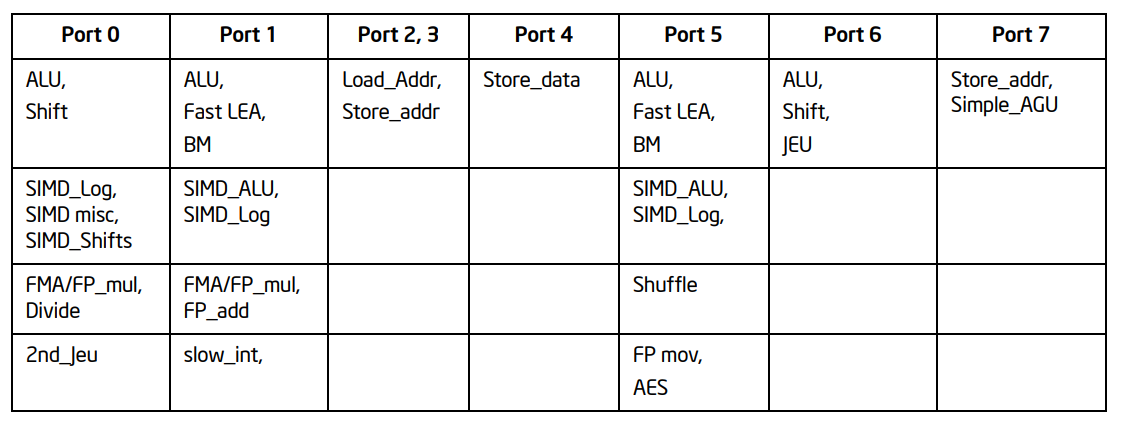
\includegraphics[width=0.49\textwidth]{tablaUnidadesEjecucion.png}
        \caption{Lista de unidades de ejecución de Haswell junto con conjuntos de instrucciones comunes que dependen de ellas.}
        \label{tablaUnidadesEjecucion}
\end{figure}

\begin{figure}[htbp]
    \centering
        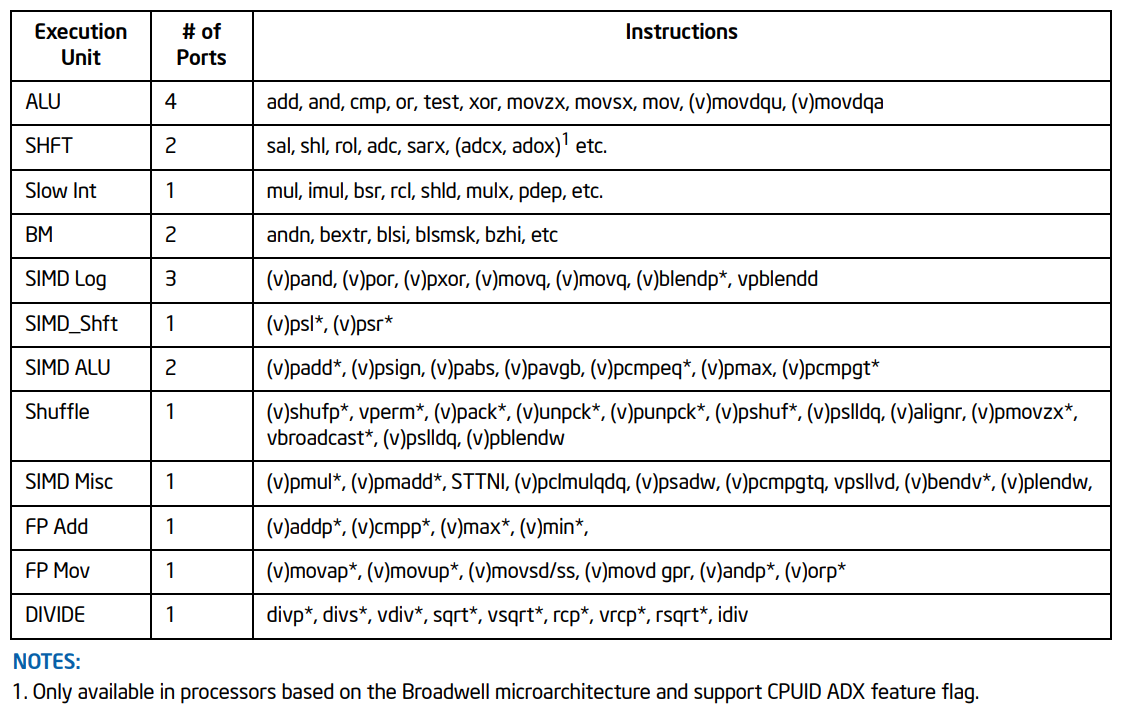
\includegraphics[width=0.49\textwidth]{tablaInstrucciones.png}
        \caption{Ejemplos de instrucciones contenidas en los conjuntos de la Figura \ref{tablaUnidadesEjecucion}.}
        \label{tablaInstrucciones}
\end{figure}

Y el total de ciclos ocupados en cada unidad de ejecución del procesador con micro-operaciones para cada uno de los bucles de los dos programas vectorizados pueden verse reflejados en los Cuadros \ref{usoPuertosMultiplicacion} y \ref{usoPuertosBucle}. Cada medida representa el número de ciclos del bucle por iteración en que la unidad de ejecución correspondiente se ha visto ocupada.

\begin{table}[htbp]
\caption{Uso de las ocho unidades de ejecución en los bucles del programa con la multiplicación vectorizada.}
    \begin{center}
    \resizebox{0.48\textwidth}{!} {
    \begin{tabular}{|c|c|c|c|c|c|c|c|c|}
    \hline
    \rowcolor[HTML]{EFEFEF} 
    \textbf{Bucle}                      & \textbf{Puerto 0} & \textbf{P. 1} & \textbf{P. 2} & \textbf{P. 3} & \textbf{P. 4} & \textbf{P. 5} & \textbf{P. 6} & \textbf{P. 7} \\ \hline
    \cellcolor[HTML]{EFEFEF}\textbf{1º} & 4.4               & 4.3               & 31.7              & 31.6              & 37.0              & 10.0              & 4.3               & 31.7              \\ \hline
    \cellcolor[HTML]{EFEFEF}\textbf{2º} & 2.0               & 5.0               & 23.0              & 23.0              & 29.0              & 4.0               & 2.0               & 23.0              \\ \hline
    \end{tabular}
    \label{usoPuertosMultiplicacion}
    }
    \end{center}
\end{table}

\begin{table}[htbp]
\caption{Uso de las ocho unidades de ejecución en los bucles del programa con la ejecución del bucle vectorizada.}
    \begin{center}
    \resizebox{0.48\textwidth}{!} {
    \begin{tabular}{|c|c|c|c|c|c|c|c|c|}
    \hline
    \rowcolor[HTML]{EFEFEF} 
    \textbf{Bucle}                      & \textbf{Puerto 0} & \textbf{P. 1} & \textbf{P. 2} & \textbf{P. 3} & \textbf{P. 4} & \textbf{P. 5} & \textbf{P. 6} & \textbf{P. 7} \\ \hline
    \cellcolor[HTML]{EFEFEF}\textbf{1º} & 14.0              & 14.0              & 71.4              & 71.3              & 81.0              & 7.0               & 7.0               & 71.3              \\ \hline
    \cellcolor[HTML]{EFEFEF}\textbf{2º} & 7.0               & 10.0              & 42.3              & 42.4              & 51.0              & 3.0               & 3.0               & 42.3              \\ \hline
    \end{tabular}
    \label{usoPuertosBucle}
    }
    \end{center}
\end{table}

Sorprendentemente, resulta que la principal carga de los bucles contenidos en el cómputo \textbf{no} es consecuencia de operaciones vectoriales, sino que se produce por la \textbf{lectura y escritura de memoria}: las unidades de ejecución 2, 3 y 4 son aquellas que se encuentran más ocupadas en todos los bucles, y tan solo ejecutan micro-operaciones relacionadas con la memoria. Consecuentemente, puede concluirse que, en el resto de programas, es probable que la mayor parte del coste de los cómputos sea consecuencia también de las operaciones efectuadas sobre la memoria.

Este elevado \textit{overhead} resultado de operaciones sobre la memoria puede ser consecuencia de los siguientes motivos:

\begin{itemize}
    \item \textbf{Primer bucle de los programas}: se están leyendo constantemente nuevos elementos de $a$ y $b$ en cada iteración del bucle, además de almacenar los cálculos en elementos también distintos de $c$.
    \item \textbf{Segundo bucle de los programas}: se están leyendo constantemente nuevos elementos de $c$; por lo menos, las escrituras en memoria se efectúan siempre sobre las mismas variables (es decir, sobre las mismas posiciones de memoria).
\end{itemize}

Además, el hecho de que en el segundo bucle de cada programa se guarde la reducción computada en los mismos elementos, en lugar de en distintas posiciones de memoria, puede ser otro  de los motivos por los cuales el segundo bucle requiere, por cada iteración, un menor número de ciclos que el primer bucle, sumado a la simplificación de la operación $c \cdot c$ adoptada a partir del código secuencial optimizado.

\section{Realización de los experimentos} \label{experimentos}

Para la realización de los experimentos, todos los códigos son compilados con el compilador de Intel \textit{ICC} y, como se ejecutarán en un procesador Haswell, se añadirá la opción \texttt{-xhaswell} para que, en caso de que el compilador lo considere óptimo, incorpore ciertas modificaciones específicas para dicha familia de procesadores.

Cada experimento se lanza a ejecución tres veces y, de cada una de estas veces, el experimento se ejecuta 10 veces distintas. Posteriormente se realiza la mediana de los valores obtenidos.

La primera implementación del código secuencial sin optimizar se compila en primera instancia del siguiente modo: \texttt{icc codigo.c -m64 -lm -msse3 -xhaswell -O0 -Wall -o codigo}; cabe destacar que la inclusión de la librería \texttt{-msse3}, a pesar de no emplear instrucciones vectoriales en los cómputos, es consecuencia de reservar memoria alineada mediante \texttt{\_mm\_malloc}, aunque no sería un requisito necesario para el funcionamiento del programa, pudiéndose emplear \texttt{malloc} en su lugar.

A mayores, se realizará otra compilación para comprobar el efecto de las optimizaciones del compilador, activando el nivel de optimización \texttt{O2} y la autovectorización de forma explícita: \texttt{icc codigo.c -m64 -lm -msse3 -xhaswell -O2 -vec -Wall -o codigo}. A partir de las opciones especificadas, es muy probable que el compilador pueda efectuar, entre otras, mejoras al código ensamblador generado como la autovectorización, la reducción global del tamaño del código (es decir, del número de instrucciones), o el desarrollo de los bucles.

Tanto la segunda implementación como las implementaciones relacionadas con las extensiones SSE se compilan del mismo modo que el código secuencial sin optimizar.: \texttt{icc codigo.c -m64 -lm -xhaswell -O0 -Wall -o codigo}. Cabe destacar que, en el caso de las implementaciones con extensiones SSE, sí es necesaria el uso de la instrucción \texttt{\_mm\_malloc} como requisito de estas últimas.

Finalmente, en el caso de la última implementación, en la cual se utiliza \textit{\textbf{OpenMP}}, será necesario incluir las librerías: \texttt{icc codigo.c -m64 -lm -msse3 -fopenmp -xhaswell -O0 -Wall -o codigo}.

\section{Resultados de los experimentos} \label{resumenExperimentos}

A partir de los experimentos realizados, pueden extraerse una serie de conclusiones sobre las ventajas y desventajas de cada una de las técnicas de programación empleadas para las implementaciones descritas anteriormente. De este modo, será posible determinar cuál o cuáles de ellas deberían ser escogidas sobre las demás de cara a futuras implementaciones en otros proyectos.

Los resultados de los experimentos realizados se muestran en las Figuras \ref{graficaq2}, \ref{graficaq4}, \ref{graficaq6} y \ref{graficaq7}. Debido a que para cómputos pequeños no se puede realizar una buena comparación entre las implementaciones estudiadas, puesto que la variabilidad de los experimentos se hace notar en gran medida por la brevedad de las regiones computacionales, todas las explicaciones se basarán en la Figura \ref{graficaq7} excepto si se especifica lo contrario.

\begin{figure}[htbp]
    \centering
        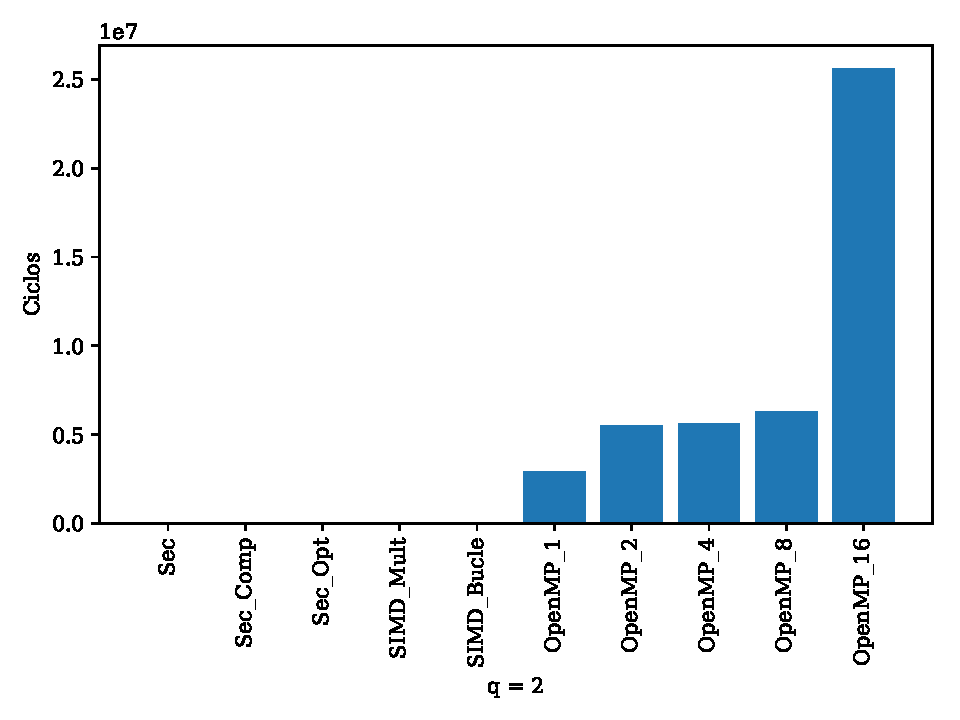
\includegraphics[width=0.48\textwidth]{graficaBarrasTandas356_2.pdf}
        \caption{Resultados de los experimentos para q = 2.}
        \label{graficaq2}
\end{figure}

\begin{figure}[htbp]
    \centering
        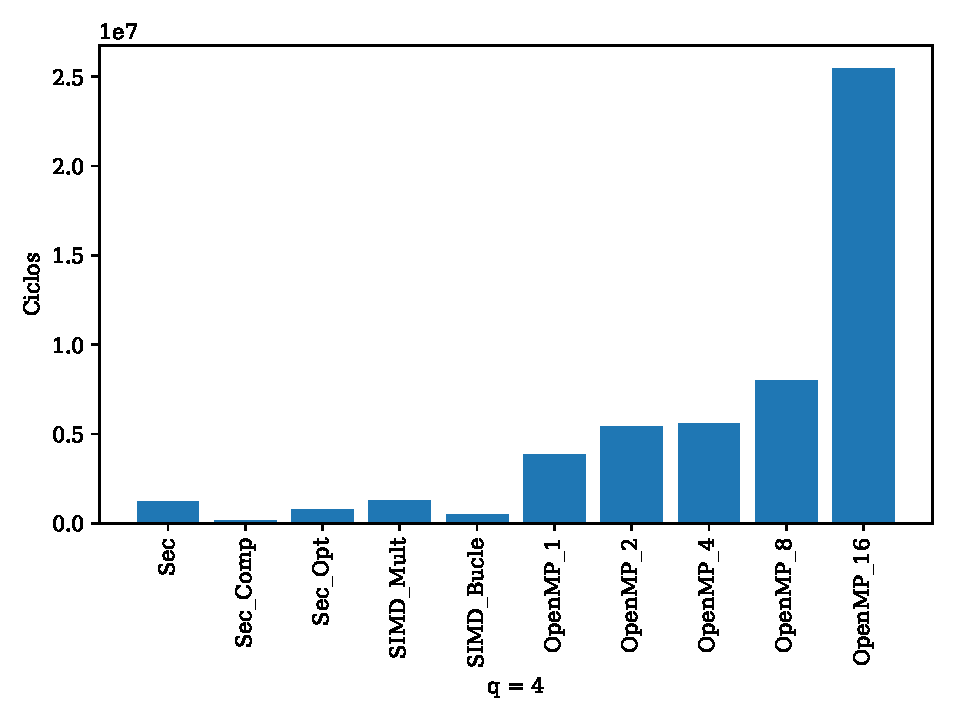
\includegraphics[width=0.48\textwidth]{graficaBarrasTandas356_4.pdf}
        \caption{Resultados de los experimentos para q = 4.}
        \label{graficaq4}
\end{figure}

\begin{figure}[htbp]
    \centering
        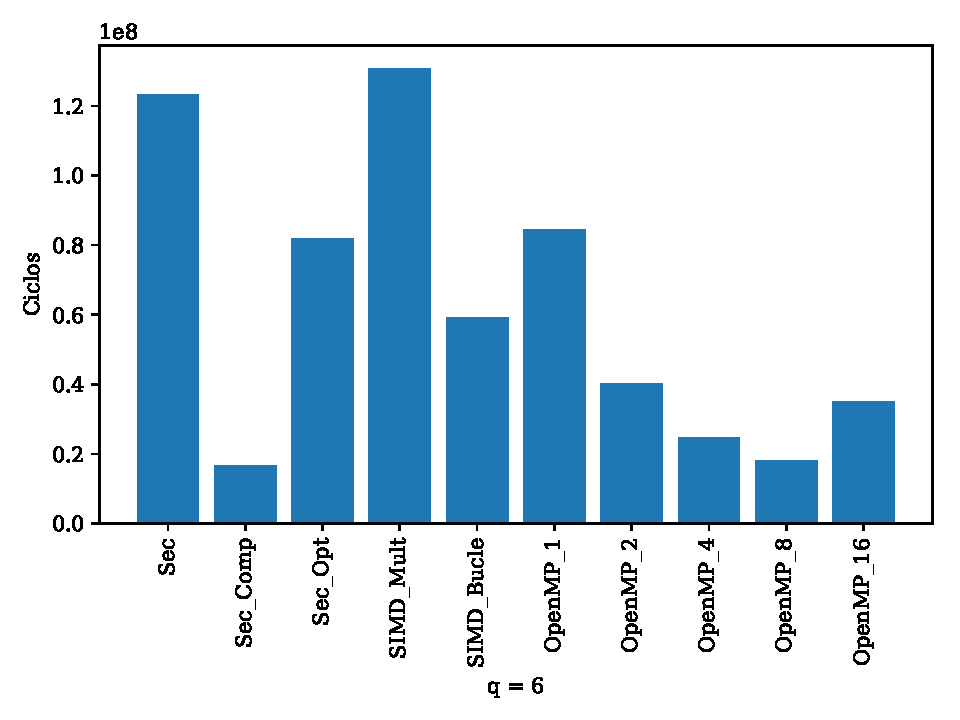
\includegraphics[width=0.48\textwidth]{graficaBarrasTandas356_6.pdf}
        \caption{Resultados de los experimentos para q = 6.}
        \label{graficaq6}
\end{figure}

\begin{figure}[htbp]
    \centering
        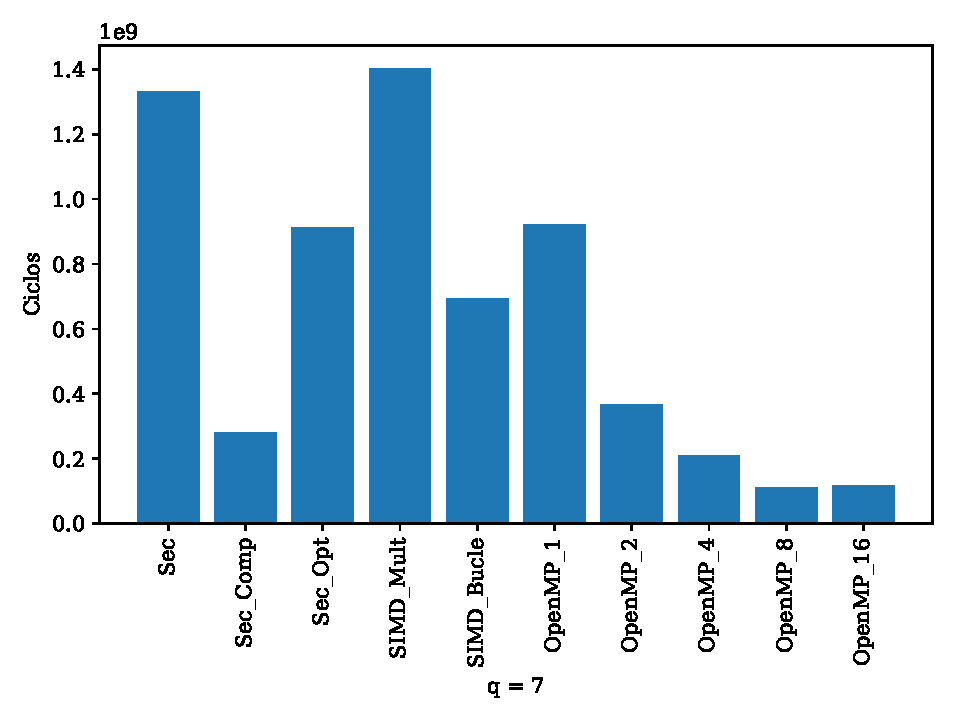
\includegraphics[width=0.48\textwidth]{graficaBarrasTandas356_7.pdf}
        \caption{Resultados de los experimentos para q = 7.}
        \label{graficaq7}
\end{figure}

\subsection{Pruebas secuenciales}
En las anteriores gráficas, el primer elemento de cada una se corresponde con el primer programa secuencial mostrado que se ha compilado sin optimizaciones por parte del compilador. Como ya se comentó previamente, este no ha sido optimizado por parte de los autores, sino que simplemente ha servido como base para los demás programas, y además para efectuar comparativas con estos últimos, los cuales se tratan de códigos desenvueltos con mayor cuidado para intentar lograr el mejor rendimiento posible.

Aunque es de esperar que este programa sea el que consume en su ejecución el mayor número de ciclos de entre todos los probados, como resultado de la falta de optimizaciones, y de la limitación de un único hilo en ejecución que realiza una única multiplicación de cuaterniones por iteración de los bucles, resulta, sin embargo, ser el segundo más lento de todos ellos. 

En contraste, el segundo elemento de las gráficas representa también el primer programa secuencial, pero esta vez con las optimizaciones que se ha indicado al compilador que efectúe automáticamente, las cuales también han sido descritas anteriormente. Sorprendentemente, el trabajo efectuado por el compilador es de tal calidad que el programa resultado es prácticamente superior a todos los demás; debe tenerse presente que este programa se ejecuta sobre un único hilo independientemente de las optimizaciones incorporadas, acercándose a aquellos programas que basan su eficiencia en la programación multihilo, como los programas que emplean 8 o 16 hilos.

El último programa secuencial es representado por el tercer elemento de las gráficas, y se trata de la versión optimizada del código base. Las sencillas optimizaciones realizadas sobre este se han comentado también previamente, y puede observarse cómo estas incurren en una notable mejora del rendimiento, reduciendo, aproximadamente, en dos terceras partes el número de ciclos necesarios.

\subsection{Pruebas con vectorización SIMD}

Continuando ahora con los programas que hacen uso de las extensiones SSE en la programación, el primero de ellos presentado es el que las emplea para vectorizar la multiplicación de dos cuaterniones. Sus resultados se encuentran representados en las gráficas por el cuarto elemento. Como recordatorio, esta propuesta trata de aprovechar la capacidad de realizar operaciones sobre cuatro números de punto flotante al mismo tiempo para para reducir el número de instrucciones a realizar en cada iteración de los bucles, aunque ejecutándose igualmente sobre un único hilo.

Desgraciadamente, el rendimiento mostrado por este programa es el peor de todos, por lo que puede concluirse que no han podido obtenerse las mejoras esperadas. De hecho, debe considerarse además la dificultad de adaptar la multiplicación de dos cuaterniones a instrucciones vectoriales, por lo que debe descartarse con más motivos como posible buena alternativa.

Por otra parte, el otro programa escrito con vectorización trataba de vectorizar la realización de las iteraciones de cada bucle, computándose en cada iteración la multiplicación de cuatro parejas de cuaterniones, ejecutándose también sobre un único hilo. Sus resultados son representados en las gráficas por el quinto elemento.

Ahora, a diferencia del anterior programa vectorial, el rendimiento mostrado es mejorado notablemente respecto al del programa secuencial mejorado (tercer elemento de las gráficas). Sin embargo, cabe destacar que la reducción de los ciclos de computación no es tan siquiera del 50\%, a pesar de intentar realizarse en cada iteración de los bucles cuatro multiplicaciones en lugar de una, y por lo tanto esperar idealmente una reducción de los ciclos a un 25\% de los originales.

De todos modos, debe considerarse que la adaptación del código base optimizado para obtener este programa vectorizado ha sido meramente trivial y, sumando al gran soporte de instrucciones vectoriales SIMD que se puede encontrar actualmente, este enfoque de programación vectorial resulta de claro interés al haber aportado los mejores resultados por el momento, sin tener en cuenta el programa optimizado optimizado por parte del compilador.

Finalmente, cabe destacar el motivo por el cual este programa vectorial sí resulta mejor que el secuencial, mientras que el otro vectorial resulta peor. Independientemente de que las instrucciones vectoriales empleadas (carga de valores, suma, resta y multiplicación) puedan suponer una mayor cantidad de ciclos respecto a sus contrapartes sin vectorización, se está aprovechando necesariamente en todo momento la capacidad de los cuaterniones de aplicar operaciones sobre los cuatro números de punto flotante que cada uno contiene. Sin embargo, es necesario recordar que, en el programa en el que se ha vectorizado la multiplicación de dos cuaterniones, existen instrucciones cuyos resultados no son aprovechados completamente.

\subsection{Pruebas con programación multihilo}

Los últimos programas sobre los cuales se han llevado experimentos son, como se ha comentado anteriormente, aquellos en los que se toma el código base optimizado y simplemente se reparte el trabajo computacional entre un número determinado de hilos que colaboran entre sí. Sus resultados se encuentran representados por los cinco últimos elementos de cada gráfica.

El primero de los elementos se trata de aquel que tan solo emplea un hilo, estando por lo tanto en una situación idéntica al del programa con el código base optimizado. Como es de esperar, los resultados son prácticamente idénticos entre ellos, solo que ligeramente mayores en el caso actual, probablemente debido en parte al \textit{overhead} inducido como como consecuencia de las directivas OpenMP incorporadas de las cuales no se va a tomar ningún partido, y en parte por la variabilidad de los resultados.

Por otra parte, los siguientes elementos se corresponden con el uso de 2, 4, 8 y 16 hilos. Como es de esperar, la existencia de una mayor cantidad de hilos en la ejecución del programa contribuyen a una menor cantidad de ciclos de procesador por parte de cada hilo. Sin embargo, la incorporación de un hilo a una ejecución con $n$ hilos no supone necesariamente una reducción del tiempo de ejecución en $\frac{1}{n+1}$ partes, lo cual sería el caso ideal. En el Cuadro \ref{factorMejoraHilo} pueden verse reflejados, para cada prueba con un número determinado de hilos, los factores de mejora ideal y real del número de ciclos respecto a la ejecución con un hilo.

\begin{table}[htbp]
\caption{Factor de mejora al aumentar los hilos}
\label{factorMejoraHilo}
\begin{center}
\begin{tabular}{
>{\columncolor[HTML]{EFEFEF}}l |c|c|c|}
\cline{2-4}
\cellcolor[HTML]{FFFFFF}                                        & \cellcolor[HTML]{EFEFEF}\textbf{Ideal} & \cellcolor[HTML]{EFEFEF}\textbf{Real} & \cellcolor[HTML]{EFEFEF}\textbf{Fracción de mejora} \\ \hline
\multicolumn{1}{|l|}{\cellcolor[HTML]{EFEFEF}\textbf{1 hilo}}   & 0.92                                   & 0.92                                  & 1                                                   \\ \hline
\multicolumn{1}{|l|}{\cellcolor[HTML]{EFEFEF}\textbf{2 hilos}}  & 0.46                                   & 0.37                                  & 2.48                                                \\ \hline
\multicolumn{1}{|l|}{\cellcolor[HTML]{EFEFEF}\textbf{4 hilos}}  & 0.23                                   & 0.21                                  & 4.38                                                \\ \hline
\multicolumn{1}{|l|}{\cellcolor[HTML]{EFEFEF}\textbf{8 hilos}}  & 0.115                                  & 0.111                                 & 8.28                                                \\ \hline
\multicolumn{1}{|l|}{\cellcolor[HTML]{EFEFEF}\textbf{16 hilos}} & 0.058                                  & 0.116                                 & 7.93                                                \\ \hline
\end{tabular}
\end{center}
\end{table}

De hecho, cabe destacar que el rendimiento obtenido para 8 y 16 hilos es prácticamente el mismo. Esto se tiene lugar, posiblemente, como consecuencia de que la carga computacional no es lo suficientemente grande como para contrarrestar los efectos negativos de la creación, gestión y destrucción del doble de hilos.

Por ello, se han realizado experimentos adicionales idénticos a los realizados hasta el momento, pero para los programas con 8 y 16 hilos exclusivamente, alcanzando ahora el valor $8$ para el parámetro $q$. La intención de ello es obtener una sección computacional de mayor carga, para forzar que esta contrarreste los efectos negativos de los hilos en el programa con 16 hilos frente al que usa 8 hilos. Los resultados de estos experimentos pueden verse reflejados en la Figura \ref{graficaOpenMP}.

\begin{figure}[htbp]
    \centering
        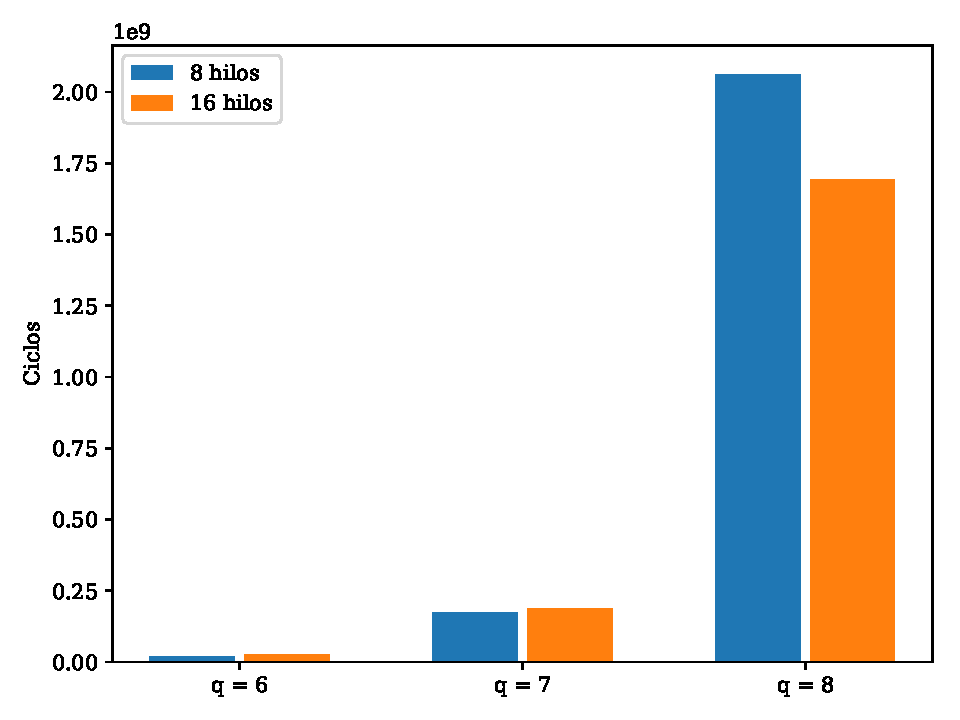
\includegraphics[width=0.48\textwidth]{graficaBarrasTanda4.pdf}
        \caption{Resultados de los experimentos para 8 y 16 hilos con OpenMP.}
        \label{graficaOpenMP}
\end{figure}

Ahora sí es posible ver un rendimiento superior en el programa con 16 hilos, aunque sin llegar a reducir notablemente los ciclos necesarios en la computación a pesar de emplear el doble de hilos, en comparación al programa que emplea 8 hilos.

Independientemente de no alcanzar las mejoras de rendimiento ideales por emplear más hilos, es innegable que al emplear hilos se obtienen rendimientos superiores frente a los programas vectoriales; además, la programación multihilo ha resultado prácticamente trivial al emplear la herramienta OpenMP. Por ello, siempre y cuando el entorno sobre el que se ejecuten los programas pongan a disposición del programador la opción de emplear ejecuciones multihilo, esta es sin duda alguna una técnica de programación que considerar para desarrollar un proyecto.

Finalmente, se analizarán ahora los datos contenidos en las gráficas para los valores $2$, $4$ y $6$ de $q$. En el caso de $q = 6$, los resultados de los experimentos de cada programa no difieren apenas de los concretados anteriormente para $q = 7$. Sin embargo, para los valores $2$ y $4$ de $q$ puede observarse cómo los programas basados en la programación multihilo dan lugar a un rendimiento incluso órdenes de magnitud inferior a los demás programas.

Debe considerarse que los ciclos de computación obtenidos para estos experimentos indican una breve duración de la región computacional, y por ello es coherente que los programas multihilo presenten unos resultados tan pésimos ya que es necesario incorporar a dicha región el coste de gestión de los hilos; de hecho, incluso el programa multihilo basado en un único hilo se ve altamente perjudicado respecto al programa secuencial con el código base mejorado, por lo que la simple inclusión de directivas OpenMP que no serán aprovechadas también supone un importante perjuicio del rendimiento.

De todos modos, la importancia de estos experimentos no es en absoluto elevada dado que es altamente improbable encontrarse en situaciones en las que la duración de las regiones computacionales de proyectos reales sean demasiado breves como para que el coste computacional de la creación de los hilos suponga una carga considerable en el rendimiento de los programas.

\section{Conclusiones}\label{conclusiones}

A partir de los experimentos realizados, se pueden extraer una serie de conclusiones acerca de los beneficios y desventajas de las técnicas de programación empleadas, así como de cuáles son algunos de los importantes factores que afectan directamente al rendimiento de un programa.

Comenzando por los dos primeros códigos, el secuencial no optimizado y el optimizado, estos demuestran que un programa puede ver su rendimiento notablemente influenciado como consecuencia de una programación poco cuidadosa. Por ejemplo, en el código no optimizado, el hecho de realizar constantemente llamadas a funciones, así como el referenciar constantemente posiciones de memoria en lugar de almacenar sus valores en variables y emplear estas, suponen, junto a otros factores, un \textit{overhead} relevante en el rendimiento del programa. Además, se tratan de pequeñas consideraciones a la hora de la programación que, con un poco de cuidado, pueden beneficiar en gran medida a un programa.

Por otra parte, cabe destacar también que el compilador puede tener un gran papel en el rendimiento de un programa, tal y como ha demostrado en la versión no optimizada del código secuencial sin optimizar. Por lo tanto, no cabe duda alguna de que, de ser posible, siempre convendría emplear las características de optimización de los compiladores a la hora de crear un programa, de cara a obtener el máximo rendimiento posible en un programa.

Tocante ahora a los programas vectorizados, pueden extraerse dos claras conclusiones a partir de ellos. En primer lugar, dada la diferencia de rendimiento de ambos programas, puede concluirse que, de cara a futuros proyectos, sería de mucho mayor interés el aprovechar las características de la programación vectorial para trabajar con grandes conjuntos de datos al mismo tiempo, tal y como se hace en la vectorización del bucle, en lugar de tratar de emplear las instrucciones vectoriales para combinar la ejecución de instrucciones no vectoriales en una vectorial, tal y como se hace en la vectorización de la multiplicación. Además, la facilidad de la adaptación del código secuencial para vectorizar la ejecución de los bucles ha resultado enormemente más simple que el proceso de vectorización de la multiplicación.

De todos modos, si se intenta aprovechar las instrucciones vectoriales para trabajar con mayores cantidades de datos al mismo tiempo, sería conveniente intentar potenciar los efectos del principio de localidad todo lo posible, tal y como se ha realizado en el programa con los bucles vectorizados al modificar la disposición de los cuaterniones en memoria.

Por lo tanto, se concluye así que la programación vectorial es una técnica cuanto menos interesante porque puede, sin duda alguna, incrementar el rendimiento de los programas de forma notable y sin requerir un gran esfuerzo en el proceso de la programación. Además, esta se encuentra disponible en un gran abanico de las CPUs empleadas hoy en día.

Finalmente, respecto a la programación multihilo, cabe destacar en primer lugar la facilidad que la librería OpenMP aporta al programador para abstraerse del manejo explícito de la creación, destrucción y control de los hilos. Al igual que con el empleo de instrucciones vectoriales para lograr la vectorización de los bucles, la adaptación del código base para ser multihilo no supone un gran esfuerzo en la programación; del mismo modo, también sería conveniente tener presentes pequeñas consideraciones, como el intentar reducir el acceso a variables compartidas por parte de los hilos y reducir así la necesidad de sincronización entre ellos, para intentar mejorar el rendimiento de los programas.

De todos modos, también se ha comprobado cómo el uso de hilos en programas que presenten pequeñas cargas computaciones no mejora el rendimiento, sino que lo empeora por el \textit{overhead} que surge como consecuencia de la creación y destrucción de hilos de ejecución. Aún así, tal y como se comentó previamente, en una situación real posiblemente no se presenten cómputos tan breves, así que esta no tiene por qué ser una importante desventaja a considerar a la hora de decidir si emplear la técnica de programación multihilo.

Por ello, puede concluirse que la programación multihilo es una técnica de interés para incrementar el rendimiento de los programas de forma notable y sin requerir un gran esfuerzo, sobre todo cuando se cuente con CPUs con un amplio soporte para la ejecución concurrente de hilos.

También debe considerarse en el caso de la programación multihilo que, en el caso de emplear un gran número de hilos, como 8 o 16, posiblemente se hubiesen obtenido también mejores factores de escalado en cuanto a rendimiento si los cómputos fuesen más extensos.

Entonces, una vez analizadas todas las técnicas de programación empleadas, podría concluirse que, en este caso en concreto, el modo de resolver el problema tratado del modo más eficiente posible consistiría en la combinación de las técnicas de vectorización, para la realización de los bucles, y de programación multihilo, todo ello sumado a la labor que el compilador podría realizar para tratar de extraer el máximo rendimiento posible de los códigos creados. El hecho de combinar dichas dos técnicas en un mismo código tiene un valor significativo: no se tratan de técnicas incompatibles, sino que deberían ser empleadas como complementarias para tratar de obtener los mejores resultados posibles.

En último lugar, aunque no relacionado directamente con las técnicas de programación empleadas, cabe recalcar los resultados obtenidos de los análisis efectuados con la herramienta IACA. Estos han mostrado cómo la mayor parte de los tiempos de cómputo de los programas vectorizados, y posiblemente de los demás también, es consecuencia directa de la gran cantidad de lecturas y escrituras de memoria que se deben realizar. Consecuentemente, se ve aquí una vez más la gran penalización de rendimiento a la que la memoria de los computadores puede llegar a dar lugar y, por tanto, la enorme importancia de intentar mejorar las prestaciones de la jerarquía de memoria.

\begin{thebibliography}{00}
\bibitem{paperOperacionesCuaterniones} Neil Dantam, ``Quaternion Computation'' [en línea]. Disponible en: \url{http://www.neil.dantam.name/note/dantam-quaternion.pdf} [fecha de consulta: 08/05/2019].
\bibitem{cesga} Centro de Supercomputación de Galicia, ``Cesga'' [en línea]. Disponible en: \url{http://www.cesga.es/} [fecha de consulta: 08/05/2019].
\bibitem{procesador} Intel Corporation, ``Intel Xeon Processor E5-2650 v3 (25M Cache, 2.30 GHz) Product Specifications'' [en línea]. Disponible en: \url{https://ark.intel.com/content/www/us/en/ark/products/81705/intel-xeon-processor-e5-2650-v3-25m-cache-2-30-ghz.html} [fecha de consulta: 08/05/2019].
\bibitem{icc} Intel Corporation, ``Intel C++ Compiler | Intel Software'' [en línea]. Disponible en: \url{https://software.intel.com/en-us/c-compilers} [fecha de consulta: 08/05/2019].
\bibitem{iacaDescarga} Intel Corporation, ``Intel Architecture Code Analyzer | Intel Software'' [en línea]. Disponible en: \url{https://software.intel.com/en-us/articles/intel-architecture-code-analyzer/} [fecha de consulta: 08/05/2019].
\bibitem{intelIntrinsics} Intel Corporation, ``Intel Intrinsics Guide'' [en línea]. Disponible en: \url{https://software.intel.com/sites/landingpage/IntrinsicsGuide/} [fecha de consulta: 08/05/2019].
\bibitem{queEsBackEnd} Jackson Marusarz, Dmitry Ryabtsev, ``Top-down Microarchitecture Analysys Method'' [en línea]. Disponible en: \url{https://software.intel.com/en-us/vtune-amplifier-cookbook-top-down-microarchitecture-analysis-method} [fecha de consulta: 12/05/2019].
\bibitem{manualIntel} Intel Corporation, ``Intel 64 and IA-32 Architectures Optimization Reference Manual'' [en línea]. Disponible en: \url{https://software.intel.com/sites/default/files/managed/9e/bc/64-ia-32-architectures-optimization-manual.pdf} [fecha de consulta: 12/05/2019].

\end{thebibliography}

\end{document}
